% =====================================================================
%  Seção da apostila: entropia da fibra do mapa aleatório de Pelikan
%  Autor: Edeilson Costa de Azevedo Filho (ICMC-USP)
%
%  Para usar na apostila:  % =====================================================================
%  Seção da apostila: entropia da fibra do mapa aleatório de Pelikan
%  Autor: Edeilson Costa de Azevedo Filho (ICMC-USP)
%
%  Para usar na apostila:  % =====================================================================
%  Seção da apostila: entropia da fibra do mapa aleatório de Pelikan
%  Autor: Edeilson Costa de Azevedo Filho (ICMC-USP)
%
%  Para usar na apostila:  % =====================================================================
%  Seção da apostila: entropia da fibra do mapa aleatório de Pelikan
%  Autor: Edeilson Costa de Azevedo Filho (ICMC-USP)
%
%  Para usar na apostila:  \input{secao_pelikan}
%  Pacotes necessários no preâmbulo da apostila:
%    amsmath, amssymb, graphicx, booktabs, hyperref, algorithm, algpseudocode
%  As figuras ficam na pasta figs/ (geradas pelo notebook do repositório).
%
\providecommand{\repoPelikan}{https://github.com/EdeilsonAzevedo/seminario-entropia-ulam}
% =====================================================================

\section{Entropia da fibra de um sistema aleatório: cálculo numérico pelo método de Ulam}
\label{sec:pelikan}

Nesta seção estudamos, de forma essencialmente numérica, a entropia da fibra de um
sistema aleatório muito simples, formado por dois mapas do intervalo: um que contrai e
outro que expande. O objetivo é mostrar como o \emph{método de Ulam} permite calcular essa
entropia e entender como ela depende da probabilidade de sortear cada mapa. Por ser um
exemplo ``controlado'', o valor exato é conhecido, o que permite validar a simulação.

Todo o código (um \emph{notebook} Jupyter que gera as figuras desta seção) e os slides da
apresentação estão disponíveis em
\begin{center}
  \url{\repoPelikan}
\end{center}

% ---------------------------------------------------------------------
\subsection{O sistema}
\label{subsec:pelikan-sistema}

\paragraph{Base.} A base é o \emph{shift} sobre as sequências de 0s e 1s:
\[
  \Omega=\{0,1\}^{\mathbb N},\qquad
  \sigma(\omega_0\omega_1\omega_2\ldots)=\omega_1\omega_2\ldots
\]
Cada símbolo é sorteado de forma independente: $\omega_k=1$ com probabilidade $p$ e
$\omega_k=0$ com probabilidade $1-p$.

\paragraph{Fibra.} A fibra é o intervalo $[0,1)$, onde agem dois mapas:
\[
  f_0(x)=\frac{x}{2}\quad\text{(contrai)},\qquad
  f_1(x)=2x \bmod 1\quad\text{(expande)}.
\]

\paragraph{Produto torcido.} O sistema completo é
\[
  F:\Omega\times[0,1)\to\Omega\times[0,1),\qquad
  F(\omega,x)=\big(\sigma\omega,\ f_{\omega_0}(x)\big).
\]
A base anda sozinha; a fibra ``obedece'' ao símbolo lido na base. Iterando,
\[
  F^n(\omega,x)=\big(\sigma^n\omega,\ f^n_\omega(x)\big),\qquad
  f^n_\omega=f_{\omega_{n-1}}\circ\cdots\circ f_{\omega_1}\circ f_{\omega_0},
\]
isto é, a cada passo o shift traz o próximo símbolo para a posição $0$, e é ele que escolhe
o mapa aplicado.

\paragraph{Notação para palavras.} Uma \emph{palavra} de tamanho $n$ é
$\omega=\omega_0\cdots\omega_{n-1}\in\{0,1\}^n$. Escrevemos
\[
  N_1(\omega)=\text{nº de 1s},\qquad N_0(\omega)=\text{nº de 0s},\qquad
  P_p(\omega)=p^{N_1(\omega)}(1-p)^{N_0(\omega)},
\]
de modo que $P_p(\omega)$ é a probabilidade de sortear a palavra $\omega$.

\paragraph{Leitura em binário.} Se $x=0{,}b_1b_2b_3\ldots$ em base 2, então
\[
  f_0(x)=0{,}0\,b_1b_2\ldots \quad\text{(insere um 0 na frente)},\qquad
  f_1(x)=0{,}b_2b_3\ldots \quad\text{(apaga o primeiro dígito)}.
\]
Essa observação simples explica quase todos os fenômenos desta seção.

\paragraph{Objetivo.} Calcular numericamente a entropia da fibra, $h_{\mathrm{fib}}(p)$,
pelo método de Ulam, e entender como ela depende de $p$.

% ---------------------------------------------------------------------
\subsection{Um alerta numérico: precisão finita}
\label{subsec:pelikan-precisao}

Antes de simular, convém notar um problema que \emph{não} é do sistema, mas do computador.
Um número em ponto flutuante de precisão dupla (\texttt{double}) guarda 53 dígitos
binários. Como $f_1$ apaga o primeiro dígito, depois de 53 aplicações de $2x\bmod1$ não
sobra dígito algum: a órbita vira exatamente $0$ e fica presa ali para sempre
(Figura~\ref{fig:pelikan-float}, à esquerda). A órbita verdadeira, calculada com
aritmética exata, continua normalmente.

\begin{figure}[ht]
  \centering
  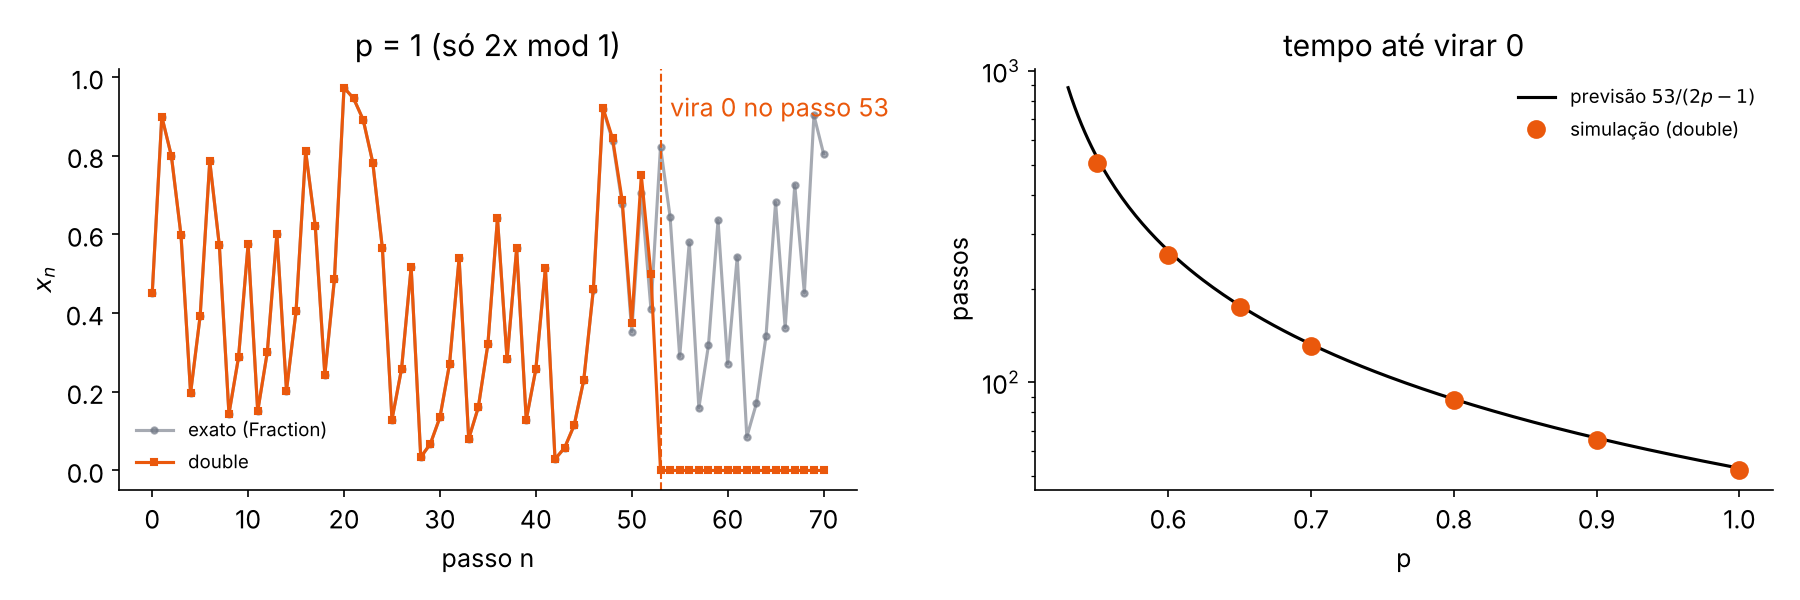
\includegraphics[width=\linewidth]{figs/f3_float.png}
  \caption{Esquerda: com $p=1$ (só $2x\bmod 1$) a órbita em \texttt{double} vira $0$ no passo 53,
  enquanto a órbita exata continua. Direita: tempo médio até a órbita em \texttt{double}
  virar $0$, comparado com a previsão $53/(2p-1)$.}
  \label{fig:pelikan-float}
\end{figure}

\paragraph{Por que $53/(2p-1)$.} Com probabilidade $p$ sai $f_1$, que consome um dígito; com
probabilidade $1-p$ sai $f_0$, que apenas insere um zero, que será apagado ``de graça''
depois. Em média, cada passo consome
\[
  p\cdot(+1)+(1-p)\cdot(-1)=2p-1
\]
dígitos. Com 53 dígitos disponíveis, a órbita dura cerca de $53/(2p-1)$ passos
(Figura~\ref{fig:pelikan-float}, à direita). Por exemplo, para $p=0{,}7$ a previsão é
de $132$ passos, e a média medida foi $129$.

\paragraph{Mais precisão só adia.} Bibliotecas de precisão arbitrária
(\texttt{mpmath}, \texttt{Fraction}) aumentam o número de bits, mas não eliminam o problema:
com $B$ bits a órbita dura $\approx B/(2p-1)$ passos. Inversamente, para simular $T$ passos
são necessários $\approx(2p-1)\,T$ bits, que crescem sem limite
(Figura~\ref{fig:pelikan-precisao}). Com $p=0{,}7$, medimos tempos de vida de
$129$, $282$, $623$ e $1232$ passos para $53$, $113$, $250$ e $500$ bits, respectivamente.

\begin{figure}[ht]
  \centering
  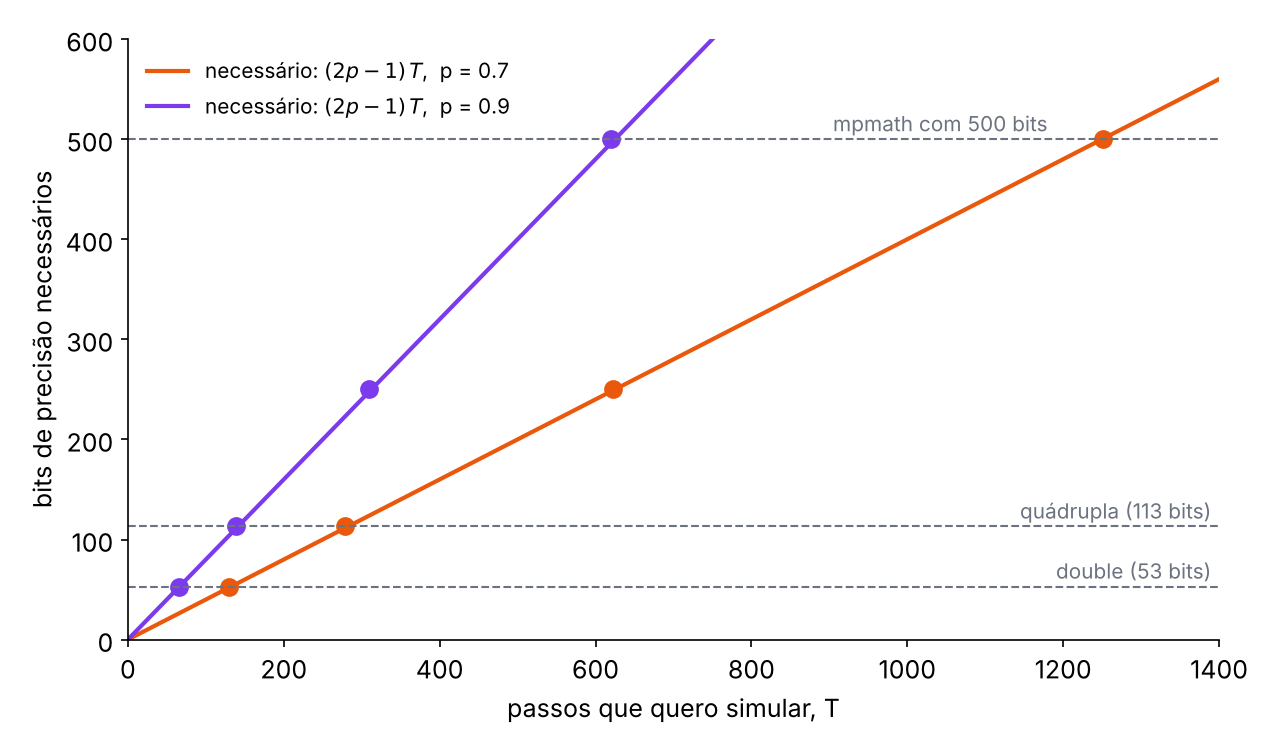
\includegraphics[width=0.7\linewidth]{figs/f3b_precisao.png}
  \caption{Bits necessários para simular $T$ passos: retas $(2p-1)\,T$ e pontos medidos com
  \texttt{mpmath}. Toda precisão fixa (linhas tracejadas) acaba sendo ultrapassada.}
  \label{fig:pelikan-precisao}
\end{figure}

\paragraph{Consequência.} Um método que precise seguir órbitas longas para estimar a entropia
não é confiável neste sistema. Precisamos de um método que use \emph{poucos passos} de cada
vez, e é isso que o método de Ulam oferece. Nas figuras de órbitas a seguir, usamos
aritmética exata.

% ---------------------------------------------------------------------
\subsection{O que sabemos e o que queremos saber}

Os casos extremos são simples:
\begin{itemize}
  \item $p=1$: só $2x\bmod1$, e a entropia da fibra é $\log 2$;
  \item $p=0$: só contração, e a entropia da fibra é $0$.
\end{itemize}
As perguntas são: o que acontece para $0<p<1$? A resposta é a média ingênua $p\log 2$?
O método de Ulam calcula $h_{\mathrm{fib}}$, e com que velocidade converge?

% ---------------------------------------------------------------------
\subsection{Comportamento das órbitas}

A Figura~\ref{fig:pelikan-traj} mostra uma órbita típica para dois valores de $p$. Com
$p=0{,}3$ a órbita cola em $0$; com $p=0{,}7$ ela percorre o intervalo todo.

\begin{figure}[ht]
  \centering
  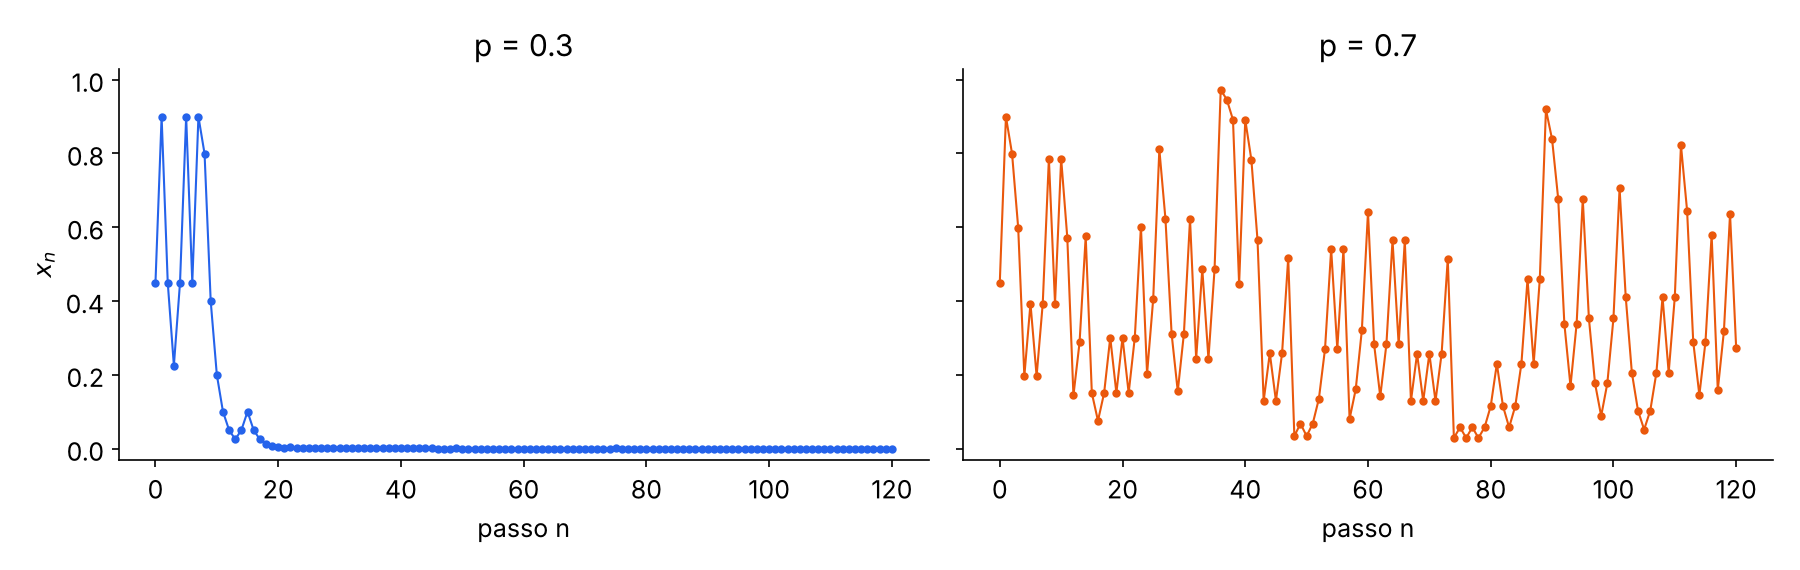
\includegraphics[width=\linewidth]{figs/f1_trajetorias.png}
  \caption{Uma órbita $x_n$ para $p=0{,}3$ (esquerda) e $p=0{,}7$ (direita).}
  \label{fig:pelikan-traj}
\end{figure}

Para entender a diferença, tomamos dois pontos quase iguais, $x_0$ e $y_0=x_0+10^{-9}$, e
aplicamos \emph{a mesma} sequência de mapas aos dois. Cada $f_1$ dobra a distância e cada
$f_0$ a divide por 2, de modo que
\[
  |x_n-y_n|\approx 2^{S_n}\,|x_0-y_0|,\qquad S_n=N_1-N_0 \text{ nos $n$ primeiros sorteios}.
\]
Com $p<\tfrac12$ as contrações vencem e os pontos se juntam: o sistema \emph{esquece} a
condição inicial (sincronização). Com $p>\tfrac12$ as expansões vencem e um erro de $10^{-9}$
cresce até o tamanho do intervalo (dependência sensível às condições iniciais). No
círculo $[0,1)$ a distância nunca passa de $\tfrac12$, por isso as curvas saturam nesse valor
(Figura~\ref{fig:pelikan-dist}).

\begin{figure}[ht]
  \centering
  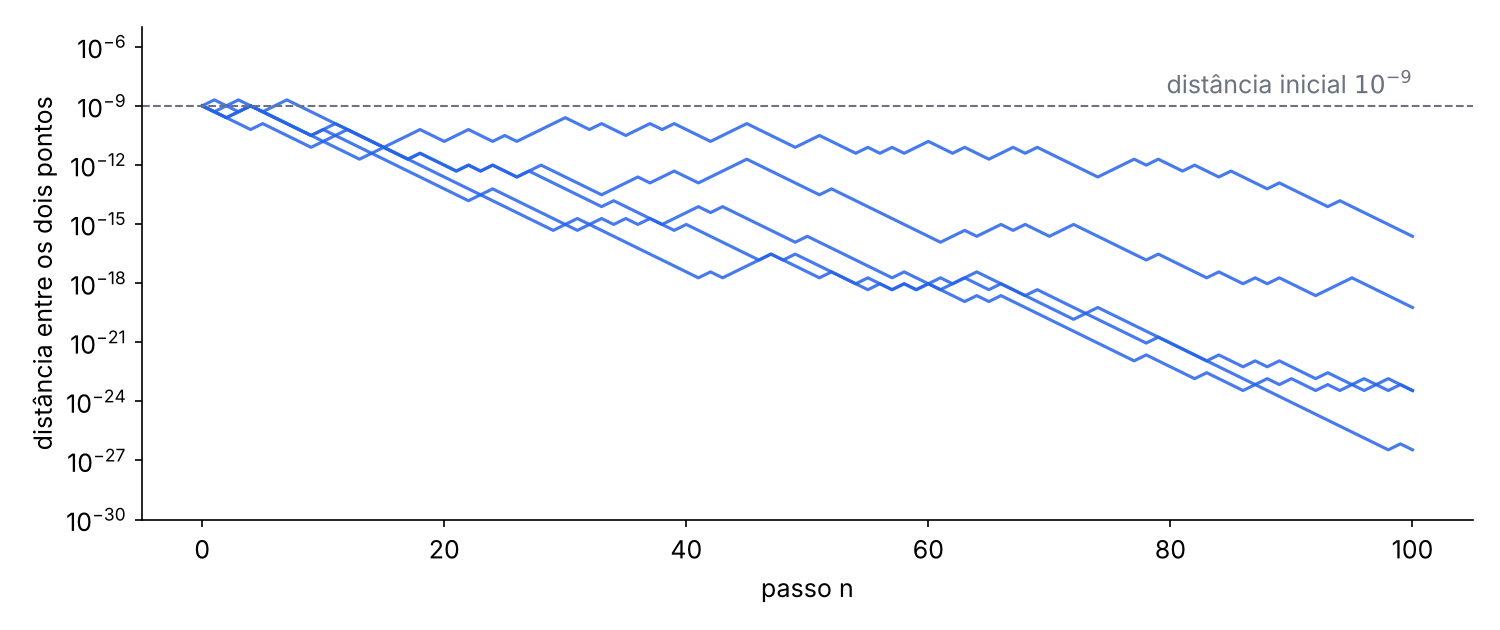
\includegraphics[width=0.49\linewidth]{figs/f2a_distancia_junta.png}\hfill
  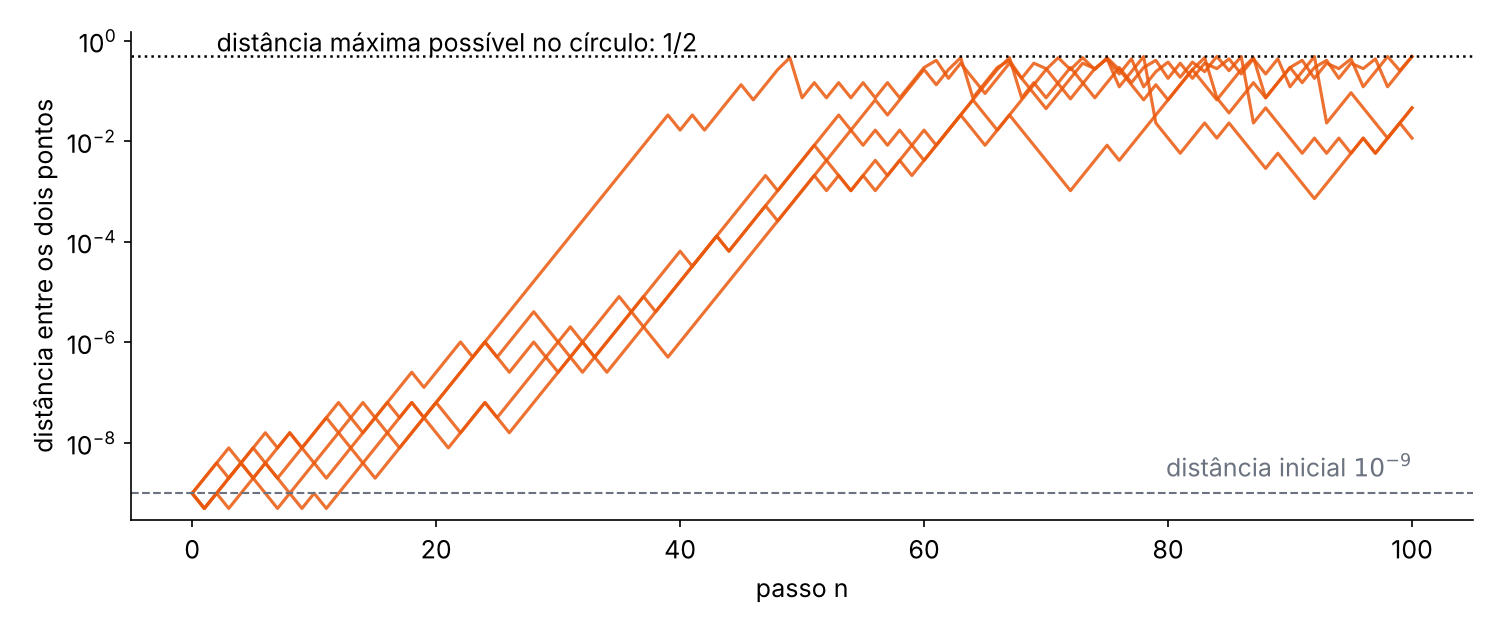
\includegraphics[width=0.49\linewidth]{figs/f2b_distancia_separa.png}
  \caption{Distância entre dois pontos inicialmente a $10^{-9}$, sob os mesmos sorteios
  (cada curva é uma sequência sorteada). Esquerda: $p=0{,}3$, os pontos se juntam.
  Direita: $p=0{,}7$, os pontos se separam até a distância máxima $\tfrac12$.}
  \label{fig:pelikan-dist}
\end{figure}

Essa é a intuição da entropia da fibra: ela mede quanta informação nova sobre $x_0$ é
preciso conhecer, a cada passo, para continuar prevendo a órbita. No regime que sincroniza,
nenhuma; no regime caótico, uma quantidade positiva.

% ---------------------------------------------------------------------
\subsection{O método de Ulam}
\label{subsec:pelikan-ulam}

Divida $[0,1)$ em $m$ células iguais $I_0,\dots,I_{m-1}$ e fixe uma palavra $\omega$ de tamanho
$n$. A \emph{matriz de Ulam} da palavra $\omega$ é
\[
  U^{(\omega)}_{ij}
  =\frac{\mathrm{Leb}\big(I_i\cap (f^n_\omega)^{-1}I_j\big)}{\mathrm{Leb}(I_i)}
  =\frac{\text{comprimento da parte de } I_i \text{ que cai em } I_j}{\text{comprimento de } I_i},
\]
ou seja, a fração da célula $i$ que termina na célula $j$ depois de aplicar os mapas de
$\omega$. Cada linha é uma distribuição de probabilidade, e sua entropia de Shannon
\[
  H_i(\omega)=-\sum_j U^{(\omega)}_{ij}\log U^{(\omega)}_{ij}
\]
mede o quanto a célula $i$ se espalhou: $H_i=0$ se ela cai inteira numa única célula e
$H_i=\log 2$ se ela se divide meio a meio entre duas. Definimos a média nas células e o
estimador de Ulam:
\[
  H(\omega)=\frac1m\sum_{i=0}^{m-1}H_i(\omega),\qquad
  \hat h_n(p)=\frac1n\sum_{\omega\in\{0,1\}^n}P_p(\omega)\,H(\omega).
\]
Note a ordem: calcula-se a entropia de cada palavra e só depois se faz a média sobre as
palavras (a sequência de sorteios é tratada como conhecida).

\begin{algorithm}[ht]
\caption{Estimador de Ulam para a entropia da fibra}
\begin{algorithmic}[1]
  \For{cada palavra $\omega$ de tamanho $n$}
    \For{cada célula $I_i$}
      \State espalhe muitos pontos dentro de $I_i$
      \State aplique os mapas de $\omega$, um por vez \Comment{0: $x/2$;\ 1: $2x\bmod 1$}
      \State $U_{ij}\gets$ fração dos pontos que terminaram em $I_j$
      \State $H_i\gets-\sum_j U_{ij}\log U_{ij}$
    \EndFor
    \State $H(\omega)\gets\frac1m\sum_i H_i$
  \EndFor
  \State \Return $\hat h_n=\frac1n\sum_\omega P_p(\omega)\,H(\omega)$
\end{algorithmic}
\end{algorithm}

Dois cuidados práticos: (i) usa-se a matriz da composição inteira $f^n_\omega$, e não o produto
de matrizes de um passo; (ii) a malha deve ser fina o bastante para $n$ passos ($m\ge 2^n$),
caso contrário a entropia de cada linha fica limitada por $\log m$ e $\hat h_n\to0$.

% ---------------------------------------------------------------------
\subsection{Exemplo com quatro células}
\label{subsec:pelikan-exemplo}

Tomemos $m=4$: $I_0=[0,\tfrac14)$, $I_1=[\tfrac14,\tfrac12)$, $I_2=[\tfrac12,\tfrac34)$,
$I_3=[\tfrac34,1)$.

\paragraph{Palavras de tamanho $n=1$.} A Tabela~\ref{tab:pelikan-n1} mostra para onde vai
cada célula. O ponto-chave é o \emph{tamanho} da imagem: $f_0$ reduz o tamanho pela metade, de
modo que a imagem ($\tfrac18$) cabe inteira numa célula; $f_1$ dobra o tamanho, de modo que a
imagem ($\tfrac12$) ocupa duas células, meio a meio.

\begin{table}[ht]
  \centering
  \small
  \begin{tabular}{cccc@{\qquad}cccc}
    \toprule
    \multicolumn{4}{c}{$f_0(x)=x/2$} & \multicolumn{4}{c}{$f_1(x)=2x\bmod 1$}\\
    \cmidrule(r){1-4}\cmidrule(l){5-8}
    célula & imagem & tam. & onde cai & célula & imagem & tam. & onde cai\\
    \midrule
    $I_0$ & $[0,\tfrac18)$ & $\tfrac18$ & $I_0$ &
    $I_0$ & $[0,\tfrac12)$ & $\tfrac12$ & $\tfrac12$ em $I_0$, $\tfrac12$ em $I_1$\\
    $I_1$ & $[\tfrac18,\tfrac14)$ & $\tfrac18$ & $I_0$ &
    $I_1$ & $[\tfrac12,1)$ & $\tfrac12$ & $\tfrac12$ em $I_2$, $\tfrac12$ em $I_3$\\
    $I_2$ & $[\tfrac14,\tfrac38)$ & $\tfrac18$ & $I_1$ &
    $I_2$ & $[0,\tfrac12)$ & $\tfrac12$ & $\tfrac12$ em $I_0$, $\tfrac12$ em $I_1$\\
    $I_3$ & $[\tfrac38,\tfrac12)$ & $\tfrac18$ & $I_1$ &
    $I_3$ & $[\tfrac12,1)$ & $\tfrac12$ & $\tfrac12$ em $I_2$, $\tfrac12$ em $I_3$\\
    \bottomrule
  \end{tabular}
  \caption{Imagens das quatro células por $f_0$ e $f_1$. Cada linha corresponde a uma linha da
  matriz de Ulam.}
  \label{tab:pelikan-n1}
\end{table}

As matrizes correspondentes são
\[
  U^{(0)}=\begin{pmatrix}1&0&0&0\\1&0&0&0\\0&1&0&0\\0&1&0&0\end{pmatrix},
  \qquad
  U^{(1)}=\begin{pmatrix}\tfrac12&\tfrac12&0&0\\0&0&\tfrac12&\tfrac12\\
  \tfrac12&\tfrac12&0&0\\0&0&\tfrac12&\tfrac12\end{pmatrix},
\]
com $H(0)=0$ e $H(1)=-2\cdot\tfrac12\log\tfrac12=\log2$. Logo
\[
  \hat h_1(p)=(1-p)\cdot 0+p\cdot\log2=p\log2 .
\]

\paragraph{Palavras de tamanho $n=2$.} Há quatro palavras:
\[
  \underbrace{\begin{pmatrix}1&0&0&0\\1&0&0&0\\1&0&0&0\\1&0&0&0\end{pmatrix}}_{\omega=00:\ x/4}
  \quad
  \underbrace{\begin{pmatrix}1&0&0&0\\0&1&0&0\\0&0&1&0\\0&0&0&1\end{pmatrix}}_{\omega=01:\ x}
  \quad
  \underbrace{\begin{pmatrix}1&0&0&0\\0&1&0&0\\1&0&0&0\\0&1&0&0\end{pmatrix}}_{\omega=10:\ \frac12(2x\bmod1)}
  \quad
  \underbrace{\begin{pmatrix}\tfrac14&\tfrac14&\tfrac14&\tfrac14\\\tfrac14&\tfrac14&\tfrac14&\tfrac14\\
  \tfrac14&\tfrac14&\tfrac14&\tfrac14\\\tfrac14&\tfrac14&\tfrac14&\tfrac14\end{pmatrix}}_{\omega=11:\ 4x\bmod1}
\]
com entropias $0$, $0$, $0$ e $\log4$, e probabilidades $(1-p)^2$, $(1-p)p$, $p(1-p)$ e $p^2$.
Portanto
\[
  \hat h_2(p)=\frac12\Big[(1-p)^2\cdot0+2p(1-p)\cdot0+p^2\cdot\log4\Big]=p^2\log2 .
\]
Repare que nas palavras $01$ e $10$ uma contração desfaz uma expansão, e nada se espalha. É por
isso que $\hat h_2<\hat h_1$: a média ingênua $p\log 2$ superestima a entropia.

% ---------------------------------------------------------------------
\subsection{Generalização: só o saldo positivo conta}
\label{subsec:pelikan-geral}

Numa palavra com $N_1(\omega)=j$ uns e $N_0(\omega)=n-j$ zeros, o mapa $f^n_\omega$ tem
inclinação $2^{S(\omega)}$ em cada célula, onde
\[
  S(\omega)=N_1(\omega)-N_0(\omega)=2j-n .
\]
A ordem dos mapas não altera o tamanho da imagem, só a contagem. Assim:
\begin{itemize}
  \item se $S(\omega)>0$, cada célula se espalha igualmente por $2^{S(\omega)}$ células, e
        $H(\omega)=-\sum 2^{-S}\log2^{-S}=S(\omega)\log 2$;
  \item se $S(\omega)\le0$, cada célula cai dentro de uma só, e $H(\omega)=0$.
\end{itemize}
Isto é, $H(\omega)=S(\omega)^+\log2$, onde $a^+=\max\{a,0\}$. Agrupando as palavras pelo número
$j$ de uns,
\[
  \hat h_n(p)=\frac1n\sum_\omega P_p(\omega)\,S(\omega)^+\log2
  =\frac{\log2}{n}\sum_{j=0}^{n}\binom nj p^j(1-p)^{n-j}\,(2j-n)^+ .
\]

\paragraph{O limite.} Se $J\sim\mathrm{Binomial}(n,p)$ é o número de uns de uma palavra
sorteada, a fórmula acima é
\[
  \hat h_n(p)=\log2\;\mathbb E\Big[\big(2\tfrac Jn-1\big)^+\Big].
\]
Pela lei dos grandes números, $J/n\to p$; como $t\mapsto(2t-1)^+$ é contínua e limitada em
$[0,1]$, obtemos
\[
  \hat h_n(p)\xrightarrow[n\to\infty]{}(2p-1)^+\log2 .
\]
Perto de $p=\tfrac12$ a convergência é lenta: $J/n$ oscila em torno de $\tfrac12$ com desvio da
ordem de $1/\sqrt n$, e a parte positiva ``aproveita'' as oscilações para cima, de modo que o
erro só decai como $1/\sqrt n$.

\paragraph{Observação.} Neste exemplo ``controlado'' há fórmula fechada e o limite coincide com
a entropia exata da fibra, $h_{\mathrm{fib}}(p)=(2p-1)^+\log2$, que pode ser obtida diretamente
pela definição contando quantos dígitos binários de $x_0$ a dinâmica revela por passo. Em
sistemas gerais não há tal fórmula, e o cálculo numérico de $\hat h_n$ é o caminho disponível.

% ---------------------------------------------------------------------
\subsection{Resultados numéricos}
\label{subsec:pelikan-resultados}

A Figura~\ref{fig:pelikan-principal} mostra $\hat h_n(p)$ para vários comprimentos de palavra.
Para $n=1$ obtemos a reta $p\log2$; conforme $n$ cresce, as curvas se aproximam de
$(2p-1)^+\log2$, que é nula até $p=\tfrac12$.

\begin{figure}[ht]
  \centering
  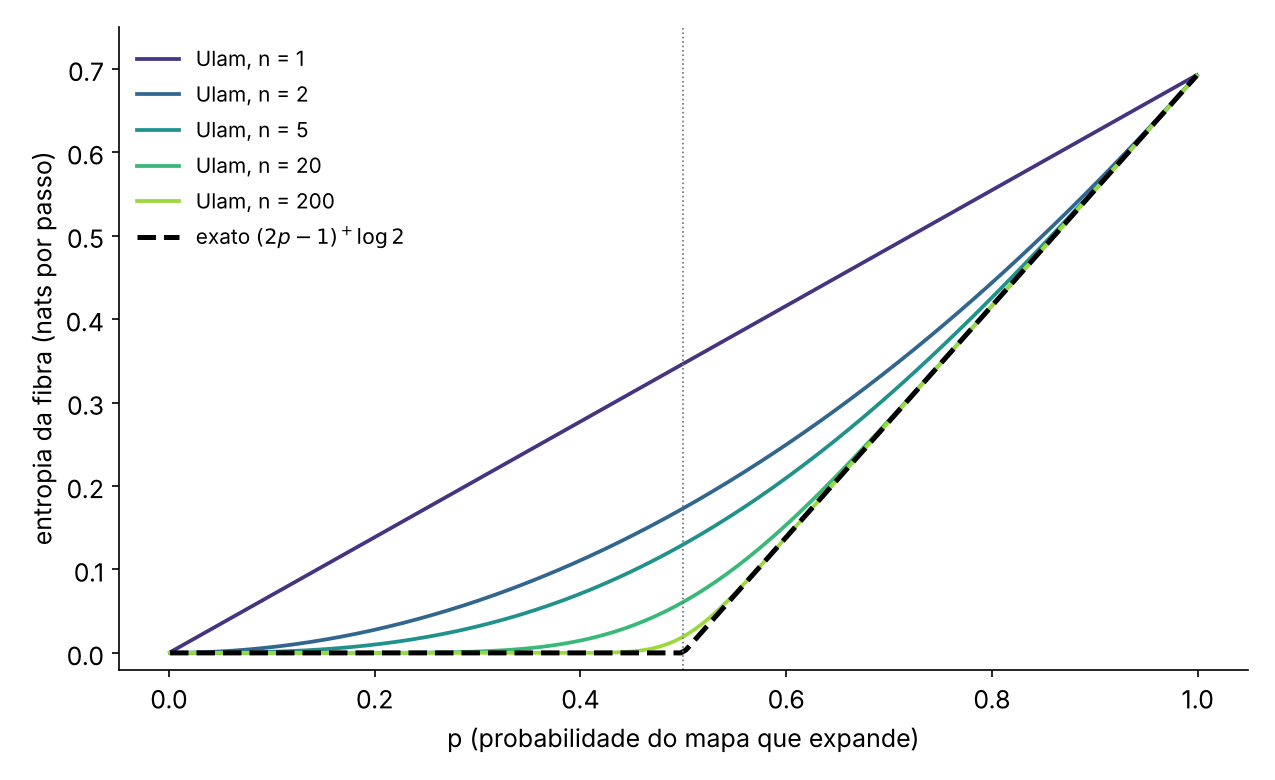
\includegraphics[width=0.72\linewidth]{figs/f7_principal.png}
  \caption{Estimador de Ulam $\hat h_n(p)$ para $n=1,2,5,20,200$ e valor exato
  $(2p-1)^+\log2$ (tracejado).}
  \label{fig:pelikan-principal}
\end{figure}

A Figura~\ref{fig:pelikan-conv} mostra a convergência em $n$ para valores fixos de $p$: longe
de $p=\tfrac12$ poucos passos bastam; em $p=\tfrac12$ a aproximação é a mais lenta.

\begin{figure}[ht]
  \centering
  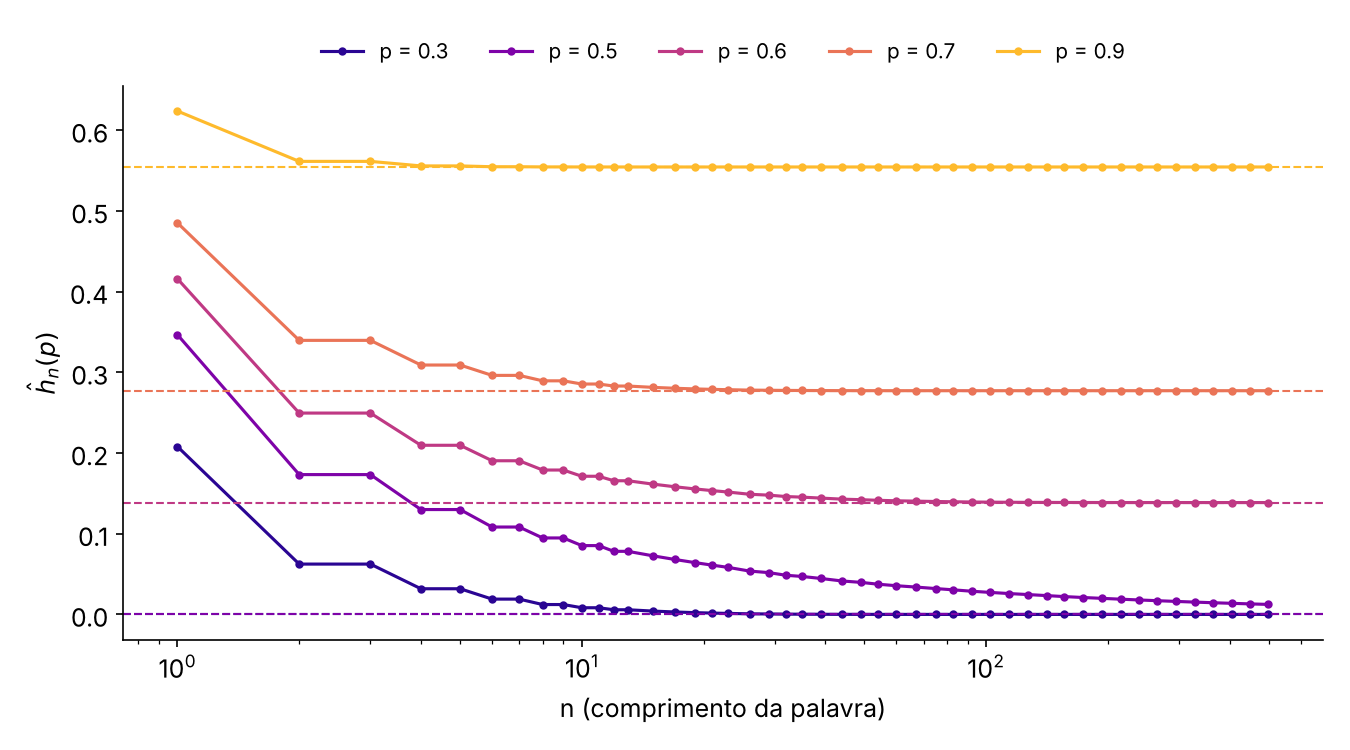
\includegraphics[width=0.75\linewidth]{figs/f9_convergencia_p.png}
  \caption{$\hat h_n(p)$ em função de $n$ para $p=0{,}3;\,0{,}5;\,0{,}6;\,0{,}7;\,0{,}9$. As linhas
  tracejadas são os valores exatos.}
  \label{fig:pelikan-conv}
\end{figure}

\paragraph{Como as curvas foram calculadas.} Para $n$ pequeno, as matrizes de Ulam foram
construídas diretamente (espalhando pontos em cada célula e aplicando os mapas). Para $n$
grande isso é inviável, pois há $2^n$ palavras; usamos então a fórmula fechada da
Seção~\ref{subsec:pelikan-geral}, que fornece \emph{exatamente} o mesmo valor que as matrizes.
A Tabela~\ref{tab:pelikan-conf} mostra a concordância para $n=4$.

\begin{table}[ht]
  \centering
  \begin{tabular}{ccc}
    \toprule
    $p$ & matrizes de Ulam ($n=4$) & fórmula fechada ($n=4$)\\
    \midrule
    0,3 & 0,03182 & 0,03182\\
    0,7 & 0,30907 & 0,30907\\
    0,9 & 0,55583 & 0,55583\\
    \bottomrule
  \end{tabular}
  \caption{Conferência entre as matrizes de Ulam construídas numericamente e a fórmula fechada.}
  \label{tab:pelikan-conf}
\end{table}

Por exemplo, para $p=0{,}7$: $\hat h_1=0{,}485$, $\hat h_2=0{,}340$, $\hat h_5=0{,}309$,
$\hat h_{20}=0{,}279$ e $\hat h_{200}=0{,}2773$, que já coincide com $0{,}4\log2\approx0{,}2773$.

% ---------------------------------------------------------------------
\subsection{Conclusões}

\begin{enumerate}
  \item \textbf{Precisão finita.} Em \texttt{double}, as órbitas deste sistema morrem em cerca de
        $53/(2p-1)$ passos; mais precisão só adia o problema. Métodos que dependem de órbitas
        longas não são confiáveis aqui.
  \item \textbf{Dois regimes.} Os mesmos dois mapas geram comportamentos opostos: para
        $p<\tfrac12$ as órbitas sincronizam, para $p>\tfrac12$ há dependência sensível. O que
        decide é o saldo entre expansões e contrações.
  \item \textbf{Método de Ulam.} O estimador mede o quanto as células se espalham usando poucos
        passos, e converge para $h_{\mathrm{fib}}(p)=(2p-1)^+\log2$, lentamente perto de
        $p=\tfrac12$. A média ingênua $p\log2$ está errada.
\end{enumerate}

% ---------------------------------------------------------------------
\subsection{Material complementar}

O repositório \url{\repoPelikan} contém:
\begin{itemize}
  \item o \emph{notebook} Jupyter que gera todas as figuras desta seção, com o código comentado e
        uma célula para experimentar outros valores de $p$ e $n$;
  \item os slides da apresentação (fonte \LaTeX{} e PDF).
\end{itemize}

\paragraph{Referências.}
\begin{itemize}
  \item Nota \emph{Ulam entropy} (material do curso), que contém a demonstração de que
        $h_{\mathrm{fib}}(p)=(2p-1)^+\log2$ e da fórmula fechada para $\hat h_n$.
  \item G.~Froyland, \emph{Ulam's method for random interval maps}, Nonlinearity \textbf{12}
        (1999), 1029--1052.
  \item C.~Monthus, \emph{Explicit dynamical properties of the Pelikan random map in the chaotic
        region and at the intermittent critical point towards the non-chaotic region},
        J.~Stat.~Mech.\ (2025), 013212.
  \item G.~Froyland, O.~Junge, G.~Ochs, \emph{Rigorous computation of topological entropy with
        respect to a finite partition}, Physica D \textbf{154} (2001), 68--84.
\end{itemize}

%  Pacotes necessários no preâmbulo da apostila:
%    amsmath, amssymb, graphicx, booktabs, hyperref, algorithm, algpseudocode
%  As figuras ficam na pasta figs/ (geradas pelo notebook do repositório).
%
\providecommand{\repoPelikan}{https://github.com/EdeilsonAzevedo/seminario-entropia-ulam}
% =====================================================================

\section{Entropia da fibra de um sistema aleatório: cálculo numérico pelo método de Ulam}
\label{sec:pelikan}

Nesta seção estudamos, de forma essencialmente numérica, a entropia da fibra de um
sistema aleatório muito simples, formado por dois mapas do intervalo: um que contrai e
outro que expande. O objetivo é mostrar como o \emph{método de Ulam} permite calcular essa
entropia e entender como ela depende da probabilidade de sortear cada mapa. Por ser um
exemplo ``controlado'', o valor exato é conhecido, o que permite validar a simulação.

Todo o código (um \emph{notebook} Jupyter que gera as figuras desta seção) e os slides da
apresentação estão disponíveis em
\begin{center}
  \url{\repoPelikan}
\end{center}

% ---------------------------------------------------------------------
\subsection{O sistema}
\label{subsec:pelikan-sistema}

\paragraph{Base.} A base é o \emph{shift} sobre as sequências de 0s e 1s:
\[
  \Omega=\{0,1\}^{\mathbb N},\qquad
  \sigma(\omega_0\omega_1\omega_2\ldots)=\omega_1\omega_2\ldots
\]
Cada símbolo é sorteado de forma independente: $\omega_k=1$ com probabilidade $p$ e
$\omega_k=0$ com probabilidade $1-p$.

\paragraph{Fibra.} A fibra é o intervalo $[0,1)$, onde agem dois mapas:
\[
  f_0(x)=\frac{x}{2}\quad\text{(contrai)},\qquad
  f_1(x)=2x \bmod 1\quad\text{(expande)}.
\]

\paragraph{Produto torcido.} O sistema completo é
\[
  F:\Omega\times[0,1)\to\Omega\times[0,1),\qquad
  F(\omega,x)=\big(\sigma\omega,\ f_{\omega_0}(x)\big).
\]
A base anda sozinha; a fibra ``obedece'' ao símbolo lido na base. Iterando,
\[
  F^n(\omega,x)=\big(\sigma^n\omega,\ f^n_\omega(x)\big),\qquad
  f^n_\omega=f_{\omega_{n-1}}\circ\cdots\circ f_{\omega_1}\circ f_{\omega_0},
\]
isto é, a cada passo o shift traz o próximo símbolo para a posição $0$, e é ele que escolhe
o mapa aplicado.

\paragraph{Notação para palavras.} Uma \emph{palavra} de tamanho $n$ é
$\omega=\omega_0\cdots\omega_{n-1}\in\{0,1\}^n$. Escrevemos
\[
  N_1(\omega)=\text{nº de 1s},\qquad N_0(\omega)=\text{nº de 0s},\qquad
  P_p(\omega)=p^{N_1(\omega)}(1-p)^{N_0(\omega)},
\]
de modo que $P_p(\omega)$ é a probabilidade de sortear a palavra $\omega$.

\paragraph{Leitura em binário.} Se $x=0{,}b_1b_2b_3\ldots$ em base 2, então
\[
  f_0(x)=0{,}0\,b_1b_2\ldots \quad\text{(insere um 0 na frente)},\qquad
  f_1(x)=0{,}b_2b_3\ldots \quad\text{(apaga o primeiro dígito)}.
\]
Essa observação simples explica quase todos os fenômenos desta seção.

\paragraph{Objetivo.} Calcular numericamente a entropia da fibra, $h_{\mathrm{fib}}(p)$,
pelo método de Ulam, e entender como ela depende de $p$.

% ---------------------------------------------------------------------
\subsection{Um alerta numérico: precisão finita}
\label{subsec:pelikan-precisao}

Antes de simular, convém notar um problema que \emph{não} é do sistema, mas do computador.
Um número em ponto flutuante de precisão dupla (\texttt{double}) guarda 53 dígitos
binários. Como $f_1$ apaga o primeiro dígito, depois de 53 aplicações de $2x\bmod1$ não
sobra dígito algum: a órbita vira exatamente $0$ e fica presa ali para sempre
(Figura~\ref{fig:pelikan-float}, à esquerda). A órbita verdadeira, calculada com
aritmética exata, continua normalmente.

\begin{figure}[ht]
  \centering
  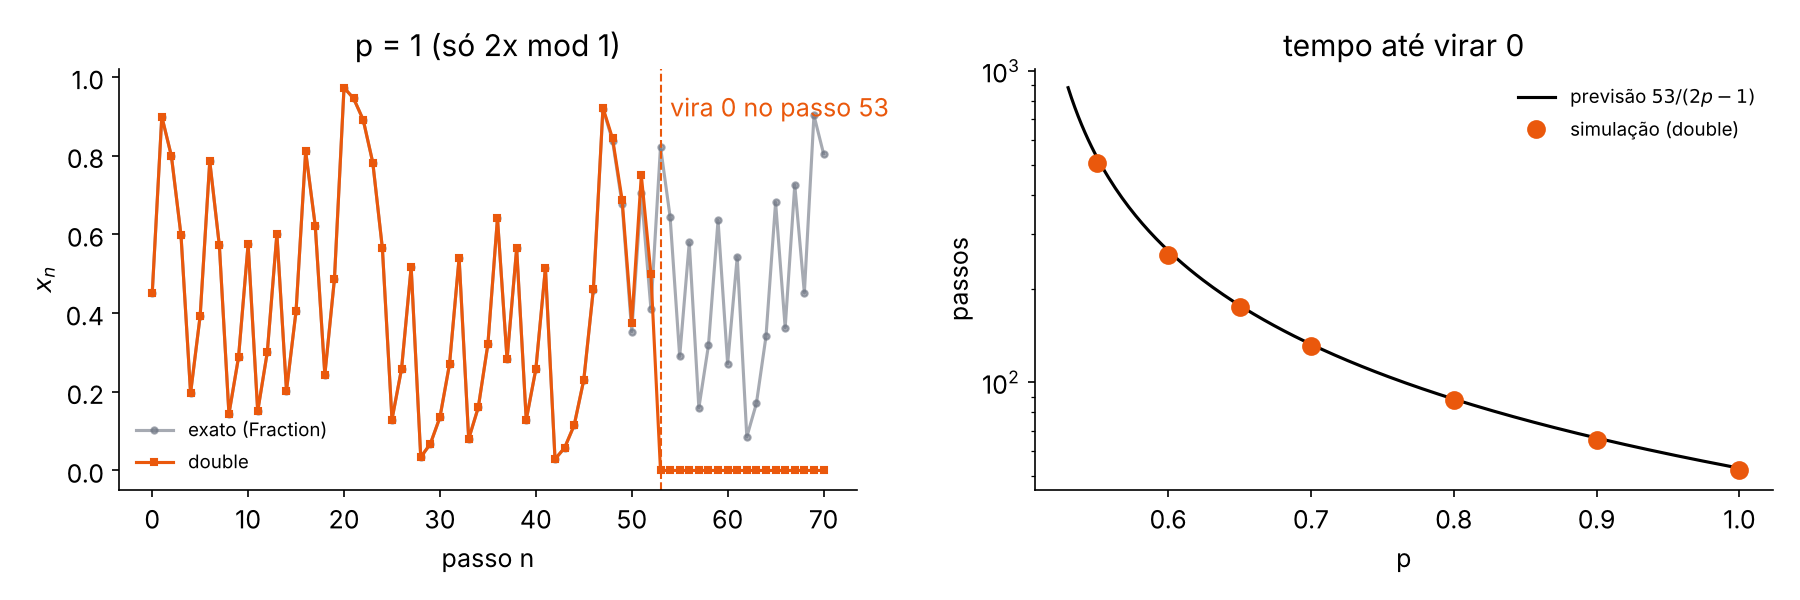
\includegraphics[width=\linewidth]{figs/f3_float.png}
  \caption{Esquerda: com $p=1$ (só $2x\bmod 1$) a órbita em \texttt{double} vira $0$ no passo 53,
  enquanto a órbita exata continua. Direita: tempo médio até a órbita em \texttt{double}
  virar $0$, comparado com a previsão $53/(2p-1)$.}
  \label{fig:pelikan-float}
\end{figure}

\paragraph{Por que $53/(2p-1)$.} Com probabilidade $p$ sai $f_1$, que consome um dígito; com
probabilidade $1-p$ sai $f_0$, que apenas insere um zero, que será apagado ``de graça''
depois. Em média, cada passo consome
\[
  p\cdot(+1)+(1-p)\cdot(-1)=2p-1
\]
dígitos. Com 53 dígitos disponíveis, a órbita dura cerca de $53/(2p-1)$ passos
(Figura~\ref{fig:pelikan-float}, à direita). Por exemplo, para $p=0{,}7$ a previsão é
de $132$ passos, e a média medida foi $129$.

\paragraph{Mais precisão só adia.} Bibliotecas de precisão arbitrária
(\texttt{mpmath}, \texttt{Fraction}) aumentam o número de bits, mas não eliminam o problema:
com $B$ bits a órbita dura $\approx B/(2p-1)$ passos. Inversamente, para simular $T$ passos
são necessários $\approx(2p-1)\,T$ bits, que crescem sem limite
(Figura~\ref{fig:pelikan-precisao}). Com $p=0{,}7$, medimos tempos de vida de
$129$, $282$, $623$ e $1232$ passos para $53$, $113$, $250$ e $500$ bits, respectivamente.

\begin{figure}[ht]
  \centering
  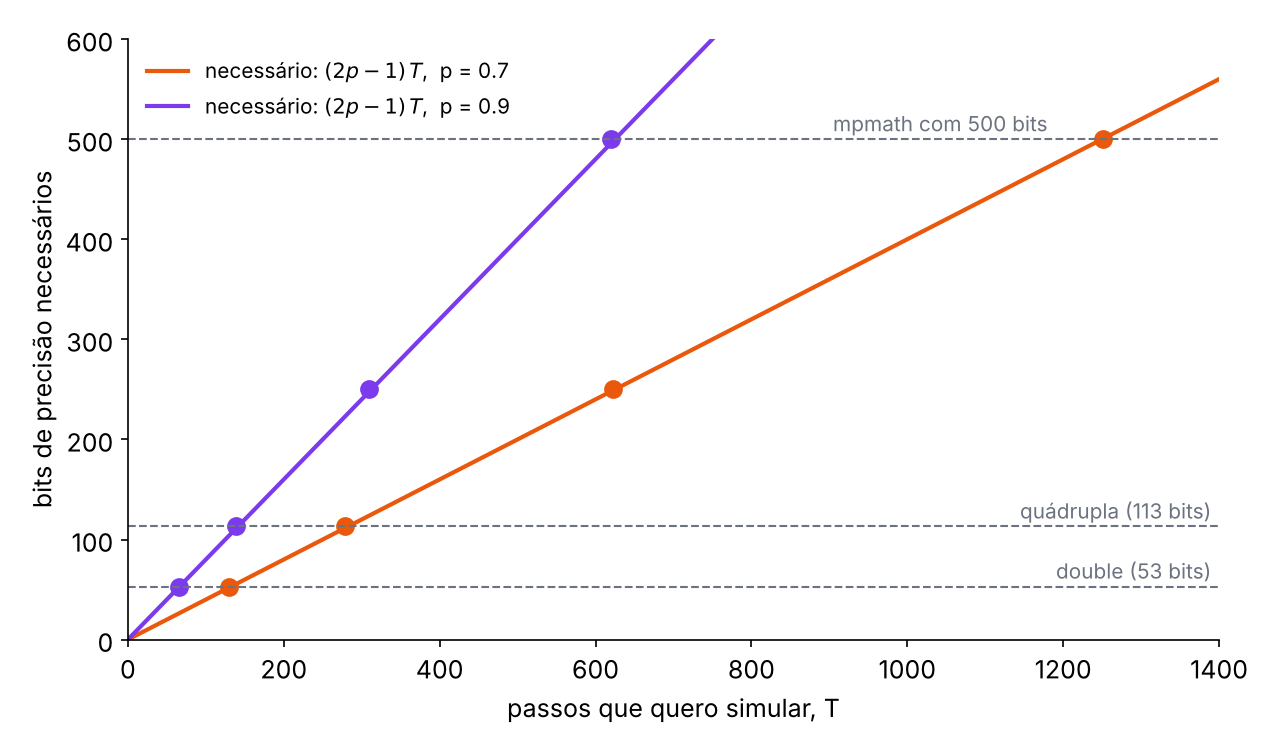
\includegraphics[width=0.7\linewidth]{figs/f3b_precisao.png}
  \caption{Bits necessários para simular $T$ passos: retas $(2p-1)\,T$ e pontos medidos com
  \texttt{mpmath}. Toda precisão fixa (linhas tracejadas) acaba sendo ultrapassada.}
  \label{fig:pelikan-precisao}
\end{figure}

\paragraph{Consequência.} Um método que precise seguir órbitas longas para estimar a entropia
não é confiável neste sistema. Precisamos de um método que use \emph{poucos passos} de cada
vez, e é isso que o método de Ulam oferece. Nas figuras de órbitas a seguir, usamos
aritmética exata.

% ---------------------------------------------------------------------
\subsection{O que sabemos e o que queremos saber}

Os casos extremos são simples:
\begin{itemize}
  \item $p=1$: só $2x\bmod1$, e a entropia da fibra é $\log 2$;
  \item $p=0$: só contração, e a entropia da fibra é $0$.
\end{itemize}
As perguntas são: o que acontece para $0<p<1$? A resposta é a média ingênua $p\log 2$?
O método de Ulam calcula $h_{\mathrm{fib}}$, e com que velocidade converge?

% ---------------------------------------------------------------------
\subsection{Comportamento das órbitas}

A Figura~\ref{fig:pelikan-traj} mostra uma órbita típica para dois valores de $p$. Com
$p=0{,}3$ a órbita cola em $0$; com $p=0{,}7$ ela percorre o intervalo todo.

\begin{figure}[ht]
  \centering
  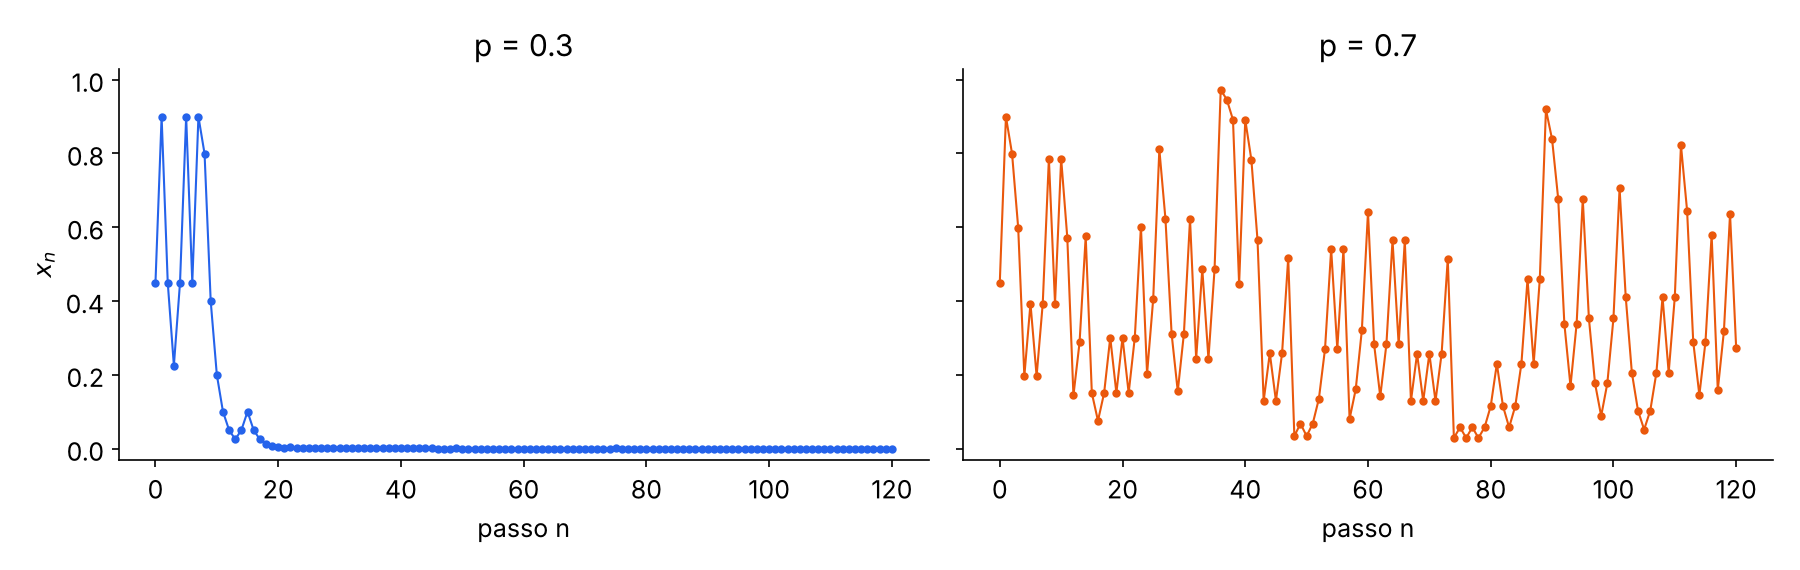
\includegraphics[width=\linewidth]{figs/f1_trajetorias.png}
  \caption{Uma órbita $x_n$ para $p=0{,}3$ (esquerda) e $p=0{,}7$ (direita).}
  \label{fig:pelikan-traj}
\end{figure}

Para entender a diferença, tomamos dois pontos quase iguais, $x_0$ e $y_0=x_0+10^{-9}$, e
aplicamos \emph{a mesma} sequência de mapas aos dois. Cada $f_1$ dobra a distância e cada
$f_0$ a divide por 2, de modo que
\[
  |x_n-y_n|\approx 2^{S_n}\,|x_0-y_0|,\qquad S_n=N_1-N_0 \text{ nos $n$ primeiros sorteios}.
\]
Com $p<\tfrac12$ as contrações vencem e os pontos se juntam: o sistema \emph{esquece} a
condição inicial (sincronização). Com $p>\tfrac12$ as expansões vencem e um erro de $10^{-9}$
cresce até o tamanho do intervalo (dependência sensível às condições iniciais). No
círculo $[0,1)$ a distância nunca passa de $\tfrac12$, por isso as curvas saturam nesse valor
(Figura~\ref{fig:pelikan-dist}).

\begin{figure}[ht]
  \centering
  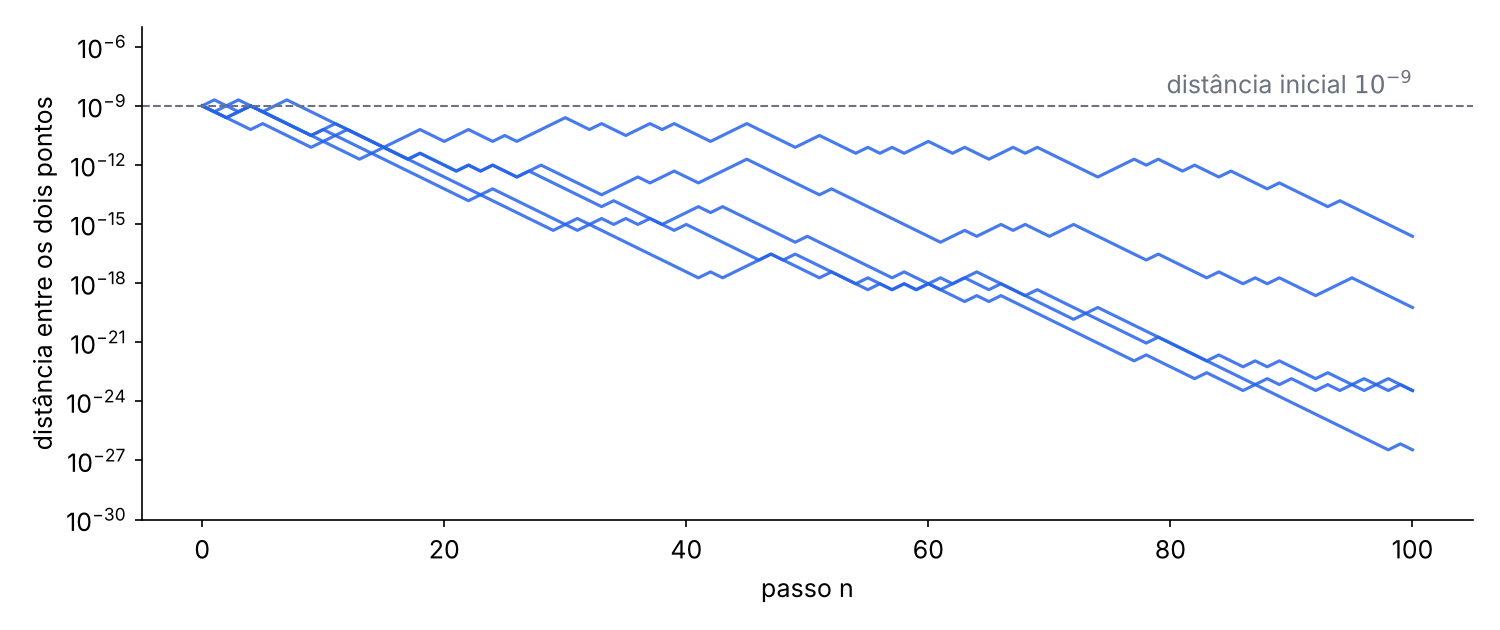
\includegraphics[width=0.49\linewidth]{figs/f2a_distancia_junta.png}\hfill
  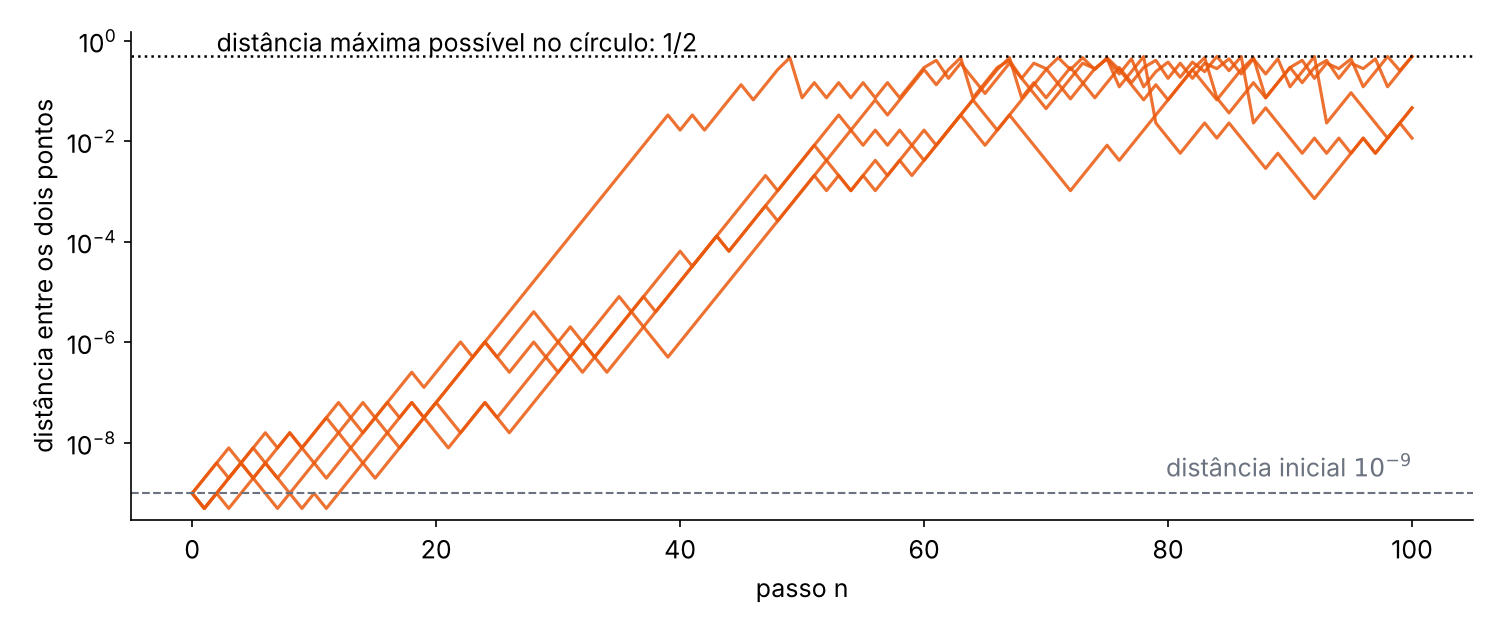
\includegraphics[width=0.49\linewidth]{figs/f2b_distancia_separa.png}
  \caption{Distância entre dois pontos inicialmente a $10^{-9}$, sob os mesmos sorteios
  (cada curva é uma sequência sorteada). Esquerda: $p=0{,}3$, os pontos se juntam.
  Direita: $p=0{,}7$, os pontos se separam até a distância máxima $\tfrac12$.}
  \label{fig:pelikan-dist}
\end{figure}

Essa é a intuição da entropia da fibra: ela mede quanta informação nova sobre $x_0$ é
preciso conhecer, a cada passo, para continuar prevendo a órbita. No regime que sincroniza,
nenhuma; no regime caótico, uma quantidade positiva.

% ---------------------------------------------------------------------
\subsection{O método de Ulam}
\label{subsec:pelikan-ulam}

Divida $[0,1)$ em $m$ células iguais $I_0,\dots,I_{m-1}$ e fixe uma palavra $\omega$ de tamanho
$n$. A \emph{matriz de Ulam} da palavra $\omega$ é
\[
  U^{(\omega)}_{ij}
  =\frac{\mathrm{Leb}\big(I_i\cap (f^n_\omega)^{-1}I_j\big)}{\mathrm{Leb}(I_i)}
  =\frac{\text{comprimento da parte de } I_i \text{ que cai em } I_j}{\text{comprimento de } I_i},
\]
ou seja, a fração da célula $i$ que termina na célula $j$ depois de aplicar os mapas de
$\omega$. Cada linha é uma distribuição de probabilidade, e sua entropia de Shannon
\[
  H_i(\omega)=-\sum_j U^{(\omega)}_{ij}\log U^{(\omega)}_{ij}
\]
mede o quanto a célula $i$ se espalhou: $H_i=0$ se ela cai inteira numa única célula e
$H_i=\log 2$ se ela se divide meio a meio entre duas. Definimos a média nas células e o
estimador de Ulam:
\[
  H(\omega)=\frac1m\sum_{i=0}^{m-1}H_i(\omega),\qquad
  \hat h_n(p)=\frac1n\sum_{\omega\in\{0,1\}^n}P_p(\omega)\,H(\omega).
\]
Note a ordem: calcula-se a entropia de cada palavra e só depois se faz a média sobre as
palavras (a sequência de sorteios é tratada como conhecida).

\begin{algorithm}[ht]
\caption{Estimador de Ulam para a entropia da fibra}
\begin{algorithmic}[1]
  \For{cada palavra $\omega$ de tamanho $n$}
    \For{cada célula $I_i$}
      \State espalhe muitos pontos dentro de $I_i$
      \State aplique os mapas de $\omega$, um por vez \Comment{0: $x/2$;\ 1: $2x\bmod 1$}
      \State $U_{ij}\gets$ fração dos pontos que terminaram em $I_j$
      \State $H_i\gets-\sum_j U_{ij}\log U_{ij}$
    \EndFor
    \State $H(\omega)\gets\frac1m\sum_i H_i$
  \EndFor
  \State \Return $\hat h_n=\frac1n\sum_\omega P_p(\omega)\,H(\omega)$
\end{algorithmic}
\end{algorithm}

Dois cuidados práticos: (i) usa-se a matriz da composição inteira $f^n_\omega$, e não o produto
de matrizes de um passo; (ii) a malha deve ser fina o bastante para $n$ passos ($m\ge 2^n$),
caso contrário a entropia de cada linha fica limitada por $\log m$ e $\hat h_n\to0$.

% ---------------------------------------------------------------------
\subsection{Exemplo com quatro células}
\label{subsec:pelikan-exemplo}

Tomemos $m=4$: $I_0=[0,\tfrac14)$, $I_1=[\tfrac14,\tfrac12)$, $I_2=[\tfrac12,\tfrac34)$,
$I_3=[\tfrac34,1)$.

\paragraph{Palavras de tamanho $n=1$.} A Tabela~\ref{tab:pelikan-n1} mostra para onde vai
cada célula. O ponto-chave é o \emph{tamanho} da imagem: $f_0$ reduz o tamanho pela metade, de
modo que a imagem ($\tfrac18$) cabe inteira numa célula; $f_1$ dobra o tamanho, de modo que a
imagem ($\tfrac12$) ocupa duas células, meio a meio.

\begin{table}[ht]
  \centering
  \small
  \begin{tabular}{cccc@{\qquad}cccc}
    \toprule
    \multicolumn{4}{c}{$f_0(x)=x/2$} & \multicolumn{4}{c}{$f_1(x)=2x\bmod 1$}\\
    \cmidrule(r){1-4}\cmidrule(l){5-8}
    célula & imagem & tam. & onde cai & célula & imagem & tam. & onde cai\\
    \midrule
    $I_0$ & $[0,\tfrac18)$ & $\tfrac18$ & $I_0$ &
    $I_0$ & $[0,\tfrac12)$ & $\tfrac12$ & $\tfrac12$ em $I_0$, $\tfrac12$ em $I_1$\\
    $I_1$ & $[\tfrac18,\tfrac14)$ & $\tfrac18$ & $I_0$ &
    $I_1$ & $[\tfrac12,1)$ & $\tfrac12$ & $\tfrac12$ em $I_2$, $\tfrac12$ em $I_3$\\
    $I_2$ & $[\tfrac14,\tfrac38)$ & $\tfrac18$ & $I_1$ &
    $I_2$ & $[0,\tfrac12)$ & $\tfrac12$ & $\tfrac12$ em $I_0$, $\tfrac12$ em $I_1$\\
    $I_3$ & $[\tfrac38,\tfrac12)$ & $\tfrac18$ & $I_1$ &
    $I_3$ & $[\tfrac12,1)$ & $\tfrac12$ & $\tfrac12$ em $I_2$, $\tfrac12$ em $I_3$\\
    \bottomrule
  \end{tabular}
  \caption{Imagens das quatro células por $f_0$ e $f_1$. Cada linha corresponde a uma linha da
  matriz de Ulam.}
  \label{tab:pelikan-n1}
\end{table}

As matrizes correspondentes são
\[
  U^{(0)}=\begin{pmatrix}1&0&0&0\\1&0&0&0\\0&1&0&0\\0&1&0&0\end{pmatrix},
  \qquad
  U^{(1)}=\begin{pmatrix}\tfrac12&\tfrac12&0&0\\0&0&\tfrac12&\tfrac12\\
  \tfrac12&\tfrac12&0&0\\0&0&\tfrac12&\tfrac12\end{pmatrix},
\]
com $H(0)=0$ e $H(1)=-2\cdot\tfrac12\log\tfrac12=\log2$. Logo
\[
  \hat h_1(p)=(1-p)\cdot 0+p\cdot\log2=p\log2 .
\]

\paragraph{Palavras de tamanho $n=2$.} Há quatro palavras:
\[
  \underbrace{\begin{pmatrix}1&0&0&0\\1&0&0&0\\1&0&0&0\\1&0&0&0\end{pmatrix}}_{\omega=00:\ x/4}
  \quad
  \underbrace{\begin{pmatrix}1&0&0&0\\0&1&0&0\\0&0&1&0\\0&0&0&1\end{pmatrix}}_{\omega=01:\ x}
  \quad
  \underbrace{\begin{pmatrix}1&0&0&0\\0&1&0&0\\1&0&0&0\\0&1&0&0\end{pmatrix}}_{\omega=10:\ \frac12(2x\bmod1)}
  \quad
  \underbrace{\begin{pmatrix}\tfrac14&\tfrac14&\tfrac14&\tfrac14\\\tfrac14&\tfrac14&\tfrac14&\tfrac14\\
  \tfrac14&\tfrac14&\tfrac14&\tfrac14\\\tfrac14&\tfrac14&\tfrac14&\tfrac14\end{pmatrix}}_{\omega=11:\ 4x\bmod1}
\]
com entropias $0$, $0$, $0$ e $\log4$, e probabilidades $(1-p)^2$, $(1-p)p$, $p(1-p)$ e $p^2$.
Portanto
\[
  \hat h_2(p)=\frac12\Big[(1-p)^2\cdot0+2p(1-p)\cdot0+p^2\cdot\log4\Big]=p^2\log2 .
\]
Repare que nas palavras $01$ e $10$ uma contração desfaz uma expansão, e nada se espalha. É por
isso que $\hat h_2<\hat h_1$: a média ingênua $p\log 2$ superestima a entropia.

% ---------------------------------------------------------------------
\subsection{Generalização: só o saldo positivo conta}
\label{subsec:pelikan-geral}

Numa palavra com $N_1(\omega)=j$ uns e $N_0(\omega)=n-j$ zeros, o mapa $f^n_\omega$ tem
inclinação $2^{S(\omega)}$ em cada célula, onde
\[
  S(\omega)=N_1(\omega)-N_0(\omega)=2j-n .
\]
A ordem dos mapas não altera o tamanho da imagem, só a contagem. Assim:
\begin{itemize}
  \item se $S(\omega)>0$, cada célula se espalha igualmente por $2^{S(\omega)}$ células, e
        $H(\omega)=-\sum 2^{-S}\log2^{-S}=S(\omega)\log 2$;
  \item se $S(\omega)\le0$, cada célula cai dentro de uma só, e $H(\omega)=0$.
\end{itemize}
Isto é, $H(\omega)=S(\omega)^+\log2$, onde $a^+=\max\{a,0\}$. Agrupando as palavras pelo número
$j$ de uns,
\[
  \hat h_n(p)=\frac1n\sum_\omega P_p(\omega)\,S(\omega)^+\log2
  =\frac{\log2}{n}\sum_{j=0}^{n}\binom nj p^j(1-p)^{n-j}\,(2j-n)^+ .
\]

\paragraph{O limite.} Se $J\sim\mathrm{Binomial}(n,p)$ é o número de uns de uma palavra
sorteada, a fórmula acima é
\[
  \hat h_n(p)=\log2\;\mathbb E\Big[\big(2\tfrac Jn-1\big)^+\Big].
\]
Pela lei dos grandes números, $J/n\to p$; como $t\mapsto(2t-1)^+$ é contínua e limitada em
$[0,1]$, obtemos
\[
  \hat h_n(p)\xrightarrow[n\to\infty]{}(2p-1)^+\log2 .
\]
Perto de $p=\tfrac12$ a convergência é lenta: $J/n$ oscila em torno de $\tfrac12$ com desvio da
ordem de $1/\sqrt n$, e a parte positiva ``aproveita'' as oscilações para cima, de modo que o
erro só decai como $1/\sqrt n$.

\paragraph{Observação.} Neste exemplo ``controlado'' há fórmula fechada e o limite coincide com
a entropia exata da fibra, $h_{\mathrm{fib}}(p)=(2p-1)^+\log2$, que pode ser obtida diretamente
pela definição contando quantos dígitos binários de $x_0$ a dinâmica revela por passo. Em
sistemas gerais não há tal fórmula, e o cálculo numérico de $\hat h_n$ é o caminho disponível.

% ---------------------------------------------------------------------
\subsection{Resultados numéricos}
\label{subsec:pelikan-resultados}

A Figura~\ref{fig:pelikan-principal} mostra $\hat h_n(p)$ para vários comprimentos de palavra.
Para $n=1$ obtemos a reta $p\log2$; conforme $n$ cresce, as curvas se aproximam de
$(2p-1)^+\log2$, que é nula até $p=\tfrac12$.

\begin{figure}[ht]
  \centering
  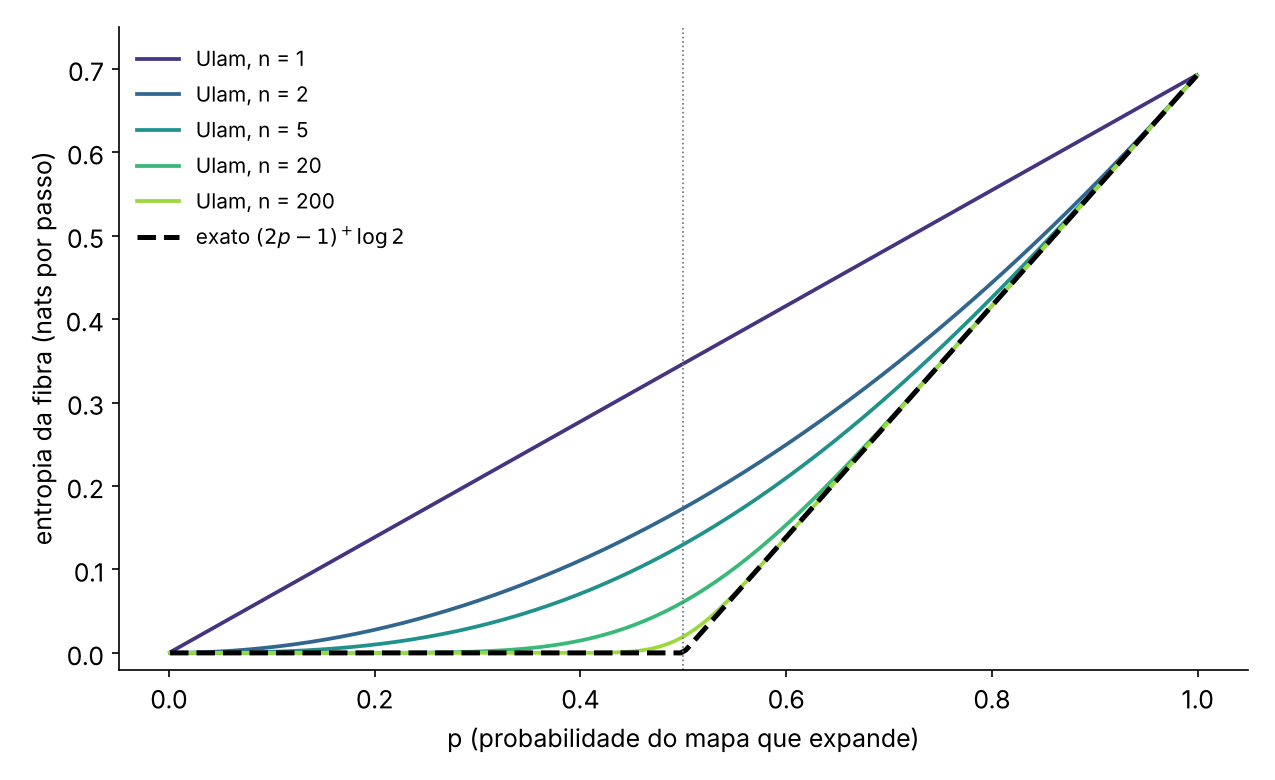
\includegraphics[width=0.72\linewidth]{figs/f7_principal.png}
  \caption{Estimador de Ulam $\hat h_n(p)$ para $n=1,2,5,20,200$ e valor exato
  $(2p-1)^+\log2$ (tracejado).}
  \label{fig:pelikan-principal}
\end{figure}

A Figura~\ref{fig:pelikan-conv} mostra a convergência em $n$ para valores fixos de $p$: longe
de $p=\tfrac12$ poucos passos bastam; em $p=\tfrac12$ a aproximação é a mais lenta.

\begin{figure}[ht]
  \centering
  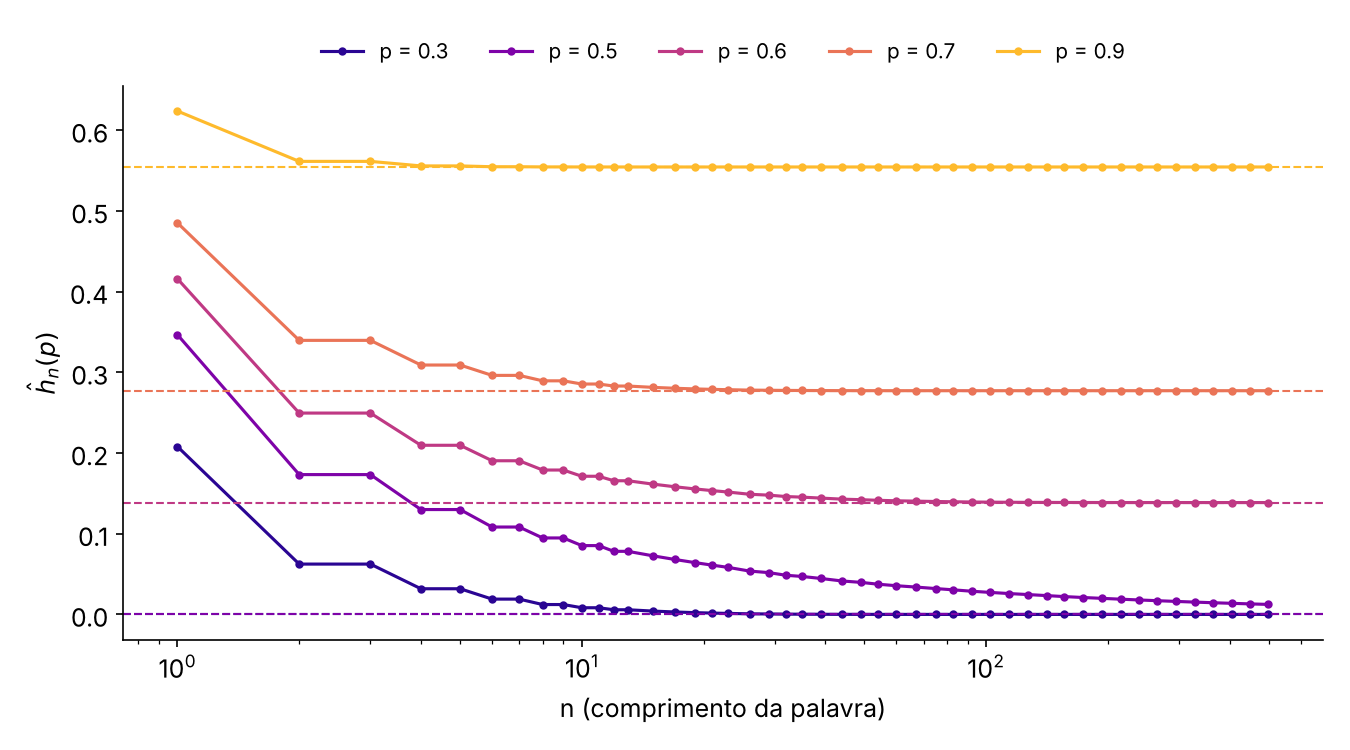
\includegraphics[width=0.75\linewidth]{figs/f9_convergencia_p.png}
  \caption{$\hat h_n(p)$ em função de $n$ para $p=0{,}3;\,0{,}5;\,0{,}6;\,0{,}7;\,0{,}9$. As linhas
  tracejadas são os valores exatos.}
  \label{fig:pelikan-conv}
\end{figure}

\paragraph{Como as curvas foram calculadas.} Para $n$ pequeno, as matrizes de Ulam foram
construídas diretamente (espalhando pontos em cada célula e aplicando os mapas). Para $n$
grande isso é inviável, pois há $2^n$ palavras; usamos então a fórmula fechada da
Seção~\ref{subsec:pelikan-geral}, que fornece \emph{exatamente} o mesmo valor que as matrizes.
A Tabela~\ref{tab:pelikan-conf} mostra a concordância para $n=4$.

\begin{table}[ht]
  \centering
  \begin{tabular}{ccc}
    \toprule
    $p$ & matrizes de Ulam ($n=4$) & fórmula fechada ($n=4$)\\
    \midrule
    0,3 & 0,03182 & 0,03182\\
    0,7 & 0,30907 & 0,30907\\
    0,9 & 0,55583 & 0,55583\\
    \bottomrule
  \end{tabular}
  \caption{Conferência entre as matrizes de Ulam construídas numericamente e a fórmula fechada.}
  \label{tab:pelikan-conf}
\end{table}

Por exemplo, para $p=0{,}7$: $\hat h_1=0{,}485$, $\hat h_2=0{,}340$, $\hat h_5=0{,}309$,
$\hat h_{20}=0{,}279$ e $\hat h_{200}=0{,}2773$, que já coincide com $0{,}4\log2\approx0{,}2773$.

% ---------------------------------------------------------------------
\subsection{Conclusões}

\begin{enumerate}
  \item \textbf{Precisão finita.} Em \texttt{double}, as órbitas deste sistema morrem em cerca de
        $53/(2p-1)$ passos; mais precisão só adia o problema. Métodos que dependem de órbitas
        longas não são confiáveis aqui.
  \item \textbf{Dois regimes.} Os mesmos dois mapas geram comportamentos opostos: para
        $p<\tfrac12$ as órbitas sincronizam, para $p>\tfrac12$ há dependência sensível. O que
        decide é o saldo entre expansões e contrações.
  \item \textbf{Método de Ulam.} O estimador mede o quanto as células se espalham usando poucos
        passos, e converge para $h_{\mathrm{fib}}(p)=(2p-1)^+\log2$, lentamente perto de
        $p=\tfrac12$. A média ingênua $p\log2$ está errada.
\end{enumerate}

% ---------------------------------------------------------------------
\subsection{Material complementar}

O repositório \url{\repoPelikan} contém:
\begin{itemize}
  \item o \emph{notebook} Jupyter que gera todas as figuras desta seção, com o código comentado e
        uma célula para experimentar outros valores de $p$ e $n$;
  \item os slides da apresentação (fonte \LaTeX{} e PDF).
\end{itemize}

\paragraph{Referências.}
\begin{itemize}
  \item Nota \emph{Ulam entropy} (material do curso), que contém a demonstração de que
        $h_{\mathrm{fib}}(p)=(2p-1)^+\log2$ e da fórmula fechada para $\hat h_n$.
  \item G.~Froyland, \emph{Ulam's method for random interval maps}, Nonlinearity \textbf{12}
        (1999), 1029--1052.
  \item C.~Monthus, \emph{Explicit dynamical properties of the Pelikan random map in the chaotic
        region and at the intermittent critical point towards the non-chaotic region},
        J.~Stat.~Mech.\ (2025), 013212.
  \item G.~Froyland, O.~Junge, G.~Ochs, \emph{Rigorous computation of topological entropy with
        respect to a finite partition}, Physica D \textbf{154} (2001), 68--84.
\end{itemize}

%  Pacotes necessários no preâmbulo da apostila:
%    amsmath, amssymb, graphicx, booktabs, hyperref, algorithm, algpseudocode
%  As figuras ficam na pasta figs/ (geradas pelo notebook do repositório).
%
\providecommand{\repoPelikan}{https://github.com/EdeilsonAzevedo/seminario-entropia-ulam}
% =====================================================================

\section{Entropia da fibra de um sistema aleatório: cálculo numérico pelo método de Ulam}
\label{sec:pelikan}

Nesta seção estudamos, de forma essencialmente numérica, a entropia da fibra de um
sistema aleatório muito simples, formado por dois mapas do intervalo: um que contrai e
outro que expande. O objetivo é mostrar como o \emph{método de Ulam} permite calcular essa
entropia e entender como ela depende da probabilidade de sortear cada mapa. Por ser um
exemplo ``controlado'', o valor exato é conhecido, o que permite validar a simulação.

Todo o código (um \emph{notebook} Jupyter que gera as figuras desta seção) e os slides da
apresentação estão disponíveis em
\begin{center}
  \url{\repoPelikan}
\end{center}

% ---------------------------------------------------------------------
\subsection{O sistema}
\label{subsec:pelikan-sistema}

\paragraph{Base.} A base é o \emph{shift} sobre as sequências de 0s e 1s:
\[
  \Omega=\{0,1\}^{\mathbb N},\qquad
  \sigma(\omega_0\omega_1\omega_2\ldots)=\omega_1\omega_2\ldots
\]
Cada símbolo é sorteado de forma independente: $\omega_k=1$ com probabilidade $p$ e
$\omega_k=0$ com probabilidade $1-p$.

\paragraph{Fibra.} A fibra é o intervalo $[0,1)$, onde agem dois mapas:
\[
  f_0(x)=\frac{x}{2}\quad\text{(contrai)},\qquad
  f_1(x)=2x \bmod 1\quad\text{(expande)}.
\]

\paragraph{Produto torcido.} O sistema completo é
\[
  F:\Omega\times[0,1)\to\Omega\times[0,1),\qquad
  F(\omega,x)=\big(\sigma\omega,\ f_{\omega_0}(x)\big).
\]
A base anda sozinha; a fibra ``obedece'' ao símbolo lido na base. Iterando,
\[
  F^n(\omega,x)=\big(\sigma^n\omega,\ f^n_\omega(x)\big),\qquad
  f^n_\omega=f_{\omega_{n-1}}\circ\cdots\circ f_{\omega_1}\circ f_{\omega_0},
\]
isto é, a cada passo o shift traz o próximo símbolo para a posição $0$, e é ele que escolhe
o mapa aplicado.

\paragraph{Notação para palavras.} Uma \emph{palavra} de tamanho $n$ é
$\omega=\omega_0\cdots\omega_{n-1}\in\{0,1\}^n$. Escrevemos
\[
  N_1(\omega)=\text{nº de 1s},\qquad N_0(\omega)=\text{nº de 0s},\qquad
  P_p(\omega)=p^{N_1(\omega)}(1-p)^{N_0(\omega)},
\]
de modo que $P_p(\omega)$ é a probabilidade de sortear a palavra $\omega$.

\paragraph{Leitura em binário.} Se $x=0{,}b_1b_2b_3\ldots$ em base 2, então
\[
  f_0(x)=0{,}0\,b_1b_2\ldots \quad\text{(insere um 0 na frente)},\qquad
  f_1(x)=0{,}b_2b_3\ldots \quad\text{(apaga o primeiro dígito)}.
\]
Essa observação simples explica quase todos os fenômenos desta seção.

\paragraph{Objetivo.} Calcular numericamente a entropia da fibra, $h_{\mathrm{fib}}(p)$,
pelo método de Ulam, e entender como ela depende de $p$.

% ---------------------------------------------------------------------
\subsection{Um alerta numérico: precisão finita}
\label{subsec:pelikan-precisao}

Antes de simular, convém notar um problema que \emph{não} é do sistema, mas do computador.
Um número em ponto flutuante de precisão dupla (\texttt{double}) guarda 53 dígitos
binários. Como $f_1$ apaga o primeiro dígito, depois de 53 aplicações de $2x\bmod1$ não
sobra dígito algum: a órbita vira exatamente $0$ e fica presa ali para sempre
(Figura~\ref{fig:pelikan-float}, à esquerda). A órbita verdadeira, calculada com
aritmética exata, continua normalmente.

\begin{figure}[ht]
  \centering
  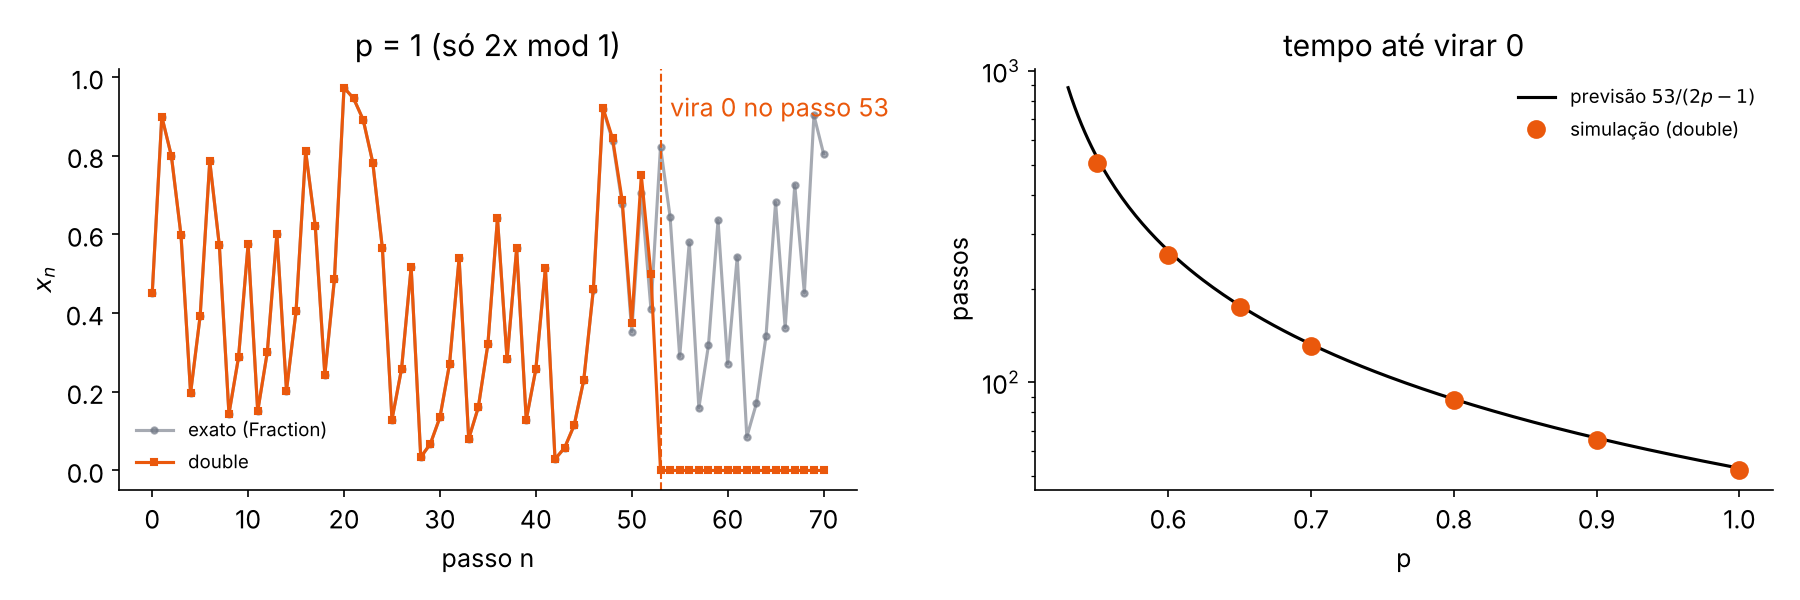
\includegraphics[width=\linewidth]{figs/f3_float.png}
  \caption{Esquerda: com $p=1$ (só $2x\bmod 1$) a órbita em \texttt{double} vira $0$ no passo 53,
  enquanto a órbita exata continua. Direita: tempo médio até a órbita em \texttt{double}
  virar $0$, comparado com a previsão $53/(2p-1)$.}
  \label{fig:pelikan-float}
\end{figure}

\paragraph{Por que $53/(2p-1)$.} Com probabilidade $p$ sai $f_1$, que consome um dígito; com
probabilidade $1-p$ sai $f_0$, que apenas insere um zero, que será apagado ``de graça''
depois. Em média, cada passo consome
\[
  p\cdot(+1)+(1-p)\cdot(-1)=2p-1
\]
dígitos. Com 53 dígitos disponíveis, a órbita dura cerca de $53/(2p-1)$ passos
(Figura~\ref{fig:pelikan-float}, à direita). Por exemplo, para $p=0{,}7$ a previsão é
de $132$ passos, e a média medida foi $129$.

\paragraph{Mais precisão só adia.} Bibliotecas de precisão arbitrária
(\texttt{mpmath}, \texttt{Fraction}) aumentam o número de bits, mas não eliminam o problema:
com $B$ bits a órbita dura $\approx B/(2p-1)$ passos. Inversamente, para simular $T$ passos
são necessários $\approx(2p-1)\,T$ bits, que crescem sem limite
(Figura~\ref{fig:pelikan-precisao}). Com $p=0{,}7$, medimos tempos de vida de
$129$, $282$, $623$ e $1232$ passos para $53$, $113$, $250$ e $500$ bits, respectivamente.

\begin{figure}[ht]
  \centering
  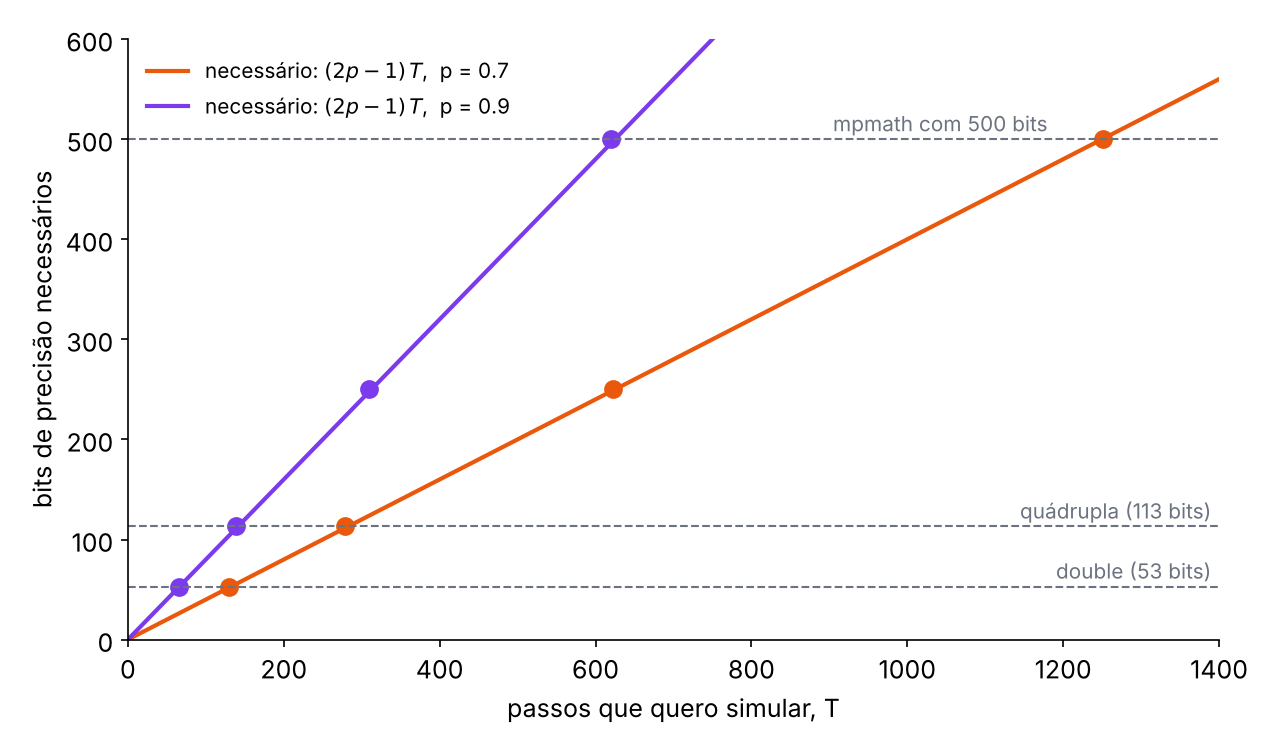
\includegraphics[width=0.7\linewidth]{figs/f3b_precisao.png}
  \caption{Bits necessários para simular $T$ passos: retas $(2p-1)\,T$ e pontos medidos com
  \texttt{mpmath}. Toda precisão fixa (linhas tracejadas) acaba sendo ultrapassada.}
  \label{fig:pelikan-precisao}
\end{figure}

\paragraph{Consequência.} Um método que precise seguir órbitas longas para estimar a entropia
não é confiável neste sistema. Precisamos de um método que use \emph{poucos passos} de cada
vez, e é isso que o método de Ulam oferece. Nas figuras de órbitas a seguir, usamos
aritmética exata.

% ---------------------------------------------------------------------
\subsection{O que sabemos e o que queremos saber}

Os casos extremos são simples:
\begin{itemize}
  \item $p=1$: só $2x\bmod1$, e a entropia da fibra é $\log 2$;
  \item $p=0$: só contração, e a entropia da fibra é $0$.
\end{itemize}
As perguntas são: o que acontece para $0<p<1$? A resposta é a média ingênua $p\log 2$?
O método de Ulam calcula $h_{\mathrm{fib}}$, e com que velocidade converge?

% ---------------------------------------------------------------------
\subsection{Comportamento das órbitas}

A Figura~\ref{fig:pelikan-traj} mostra uma órbita típica para dois valores de $p$. Com
$p=0{,}3$ a órbita cola em $0$; com $p=0{,}7$ ela percorre o intervalo todo.

\begin{figure}[ht]
  \centering
  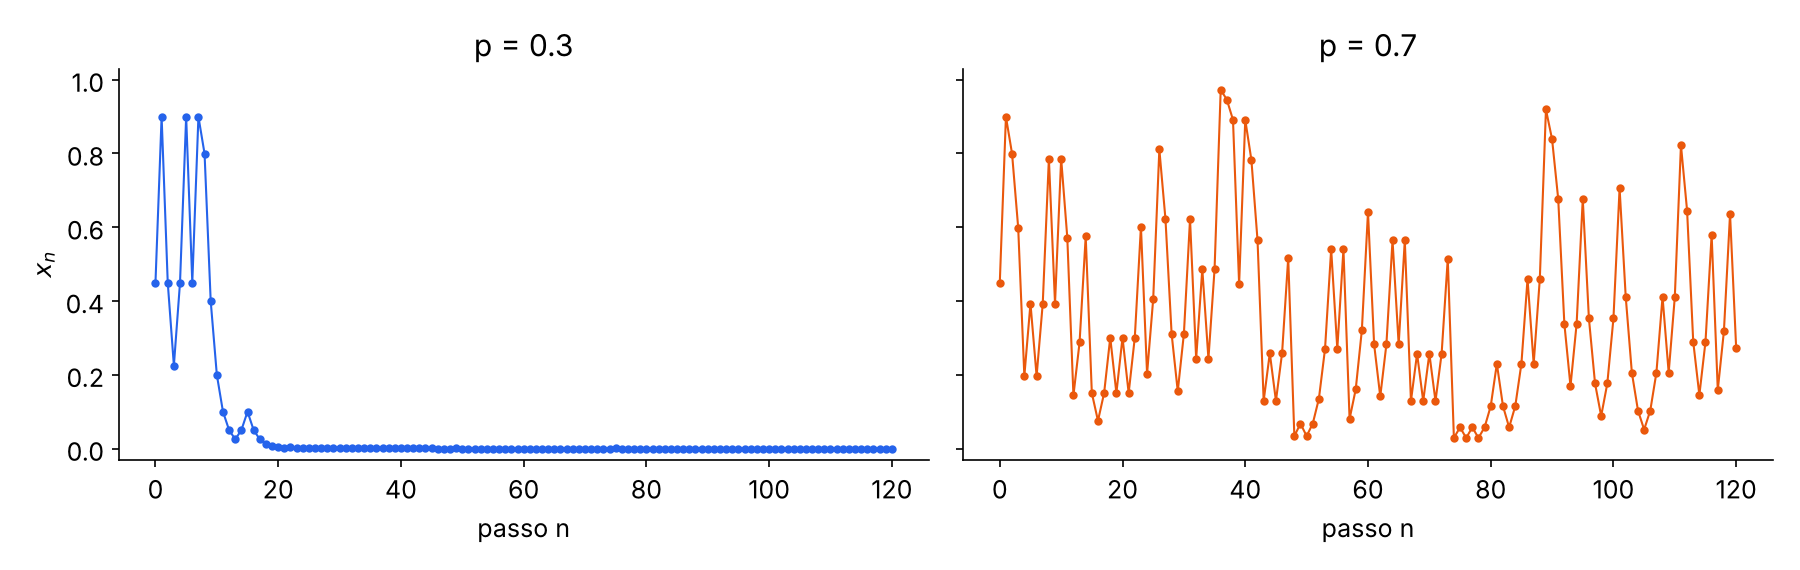
\includegraphics[width=\linewidth]{figs/f1_trajetorias.png}
  \caption{Uma órbita $x_n$ para $p=0{,}3$ (esquerda) e $p=0{,}7$ (direita).}
  \label{fig:pelikan-traj}
\end{figure}

Para entender a diferença, tomamos dois pontos quase iguais, $x_0$ e $y_0=x_0+10^{-9}$, e
aplicamos \emph{a mesma} sequência de mapas aos dois. Cada $f_1$ dobra a distância e cada
$f_0$ a divide por 2, de modo que
\[
  |x_n-y_n|\approx 2^{S_n}\,|x_0-y_0|,\qquad S_n=N_1-N_0 \text{ nos $n$ primeiros sorteios}.
\]
Com $p<\tfrac12$ as contrações vencem e os pontos se juntam: o sistema \emph{esquece} a
condição inicial (sincronização). Com $p>\tfrac12$ as expansões vencem e um erro de $10^{-9}$
cresce até o tamanho do intervalo (dependência sensível às condições iniciais). No
círculo $[0,1)$ a distância nunca passa de $\tfrac12$, por isso as curvas saturam nesse valor
(Figura~\ref{fig:pelikan-dist}).

\begin{figure}[ht]
  \centering
  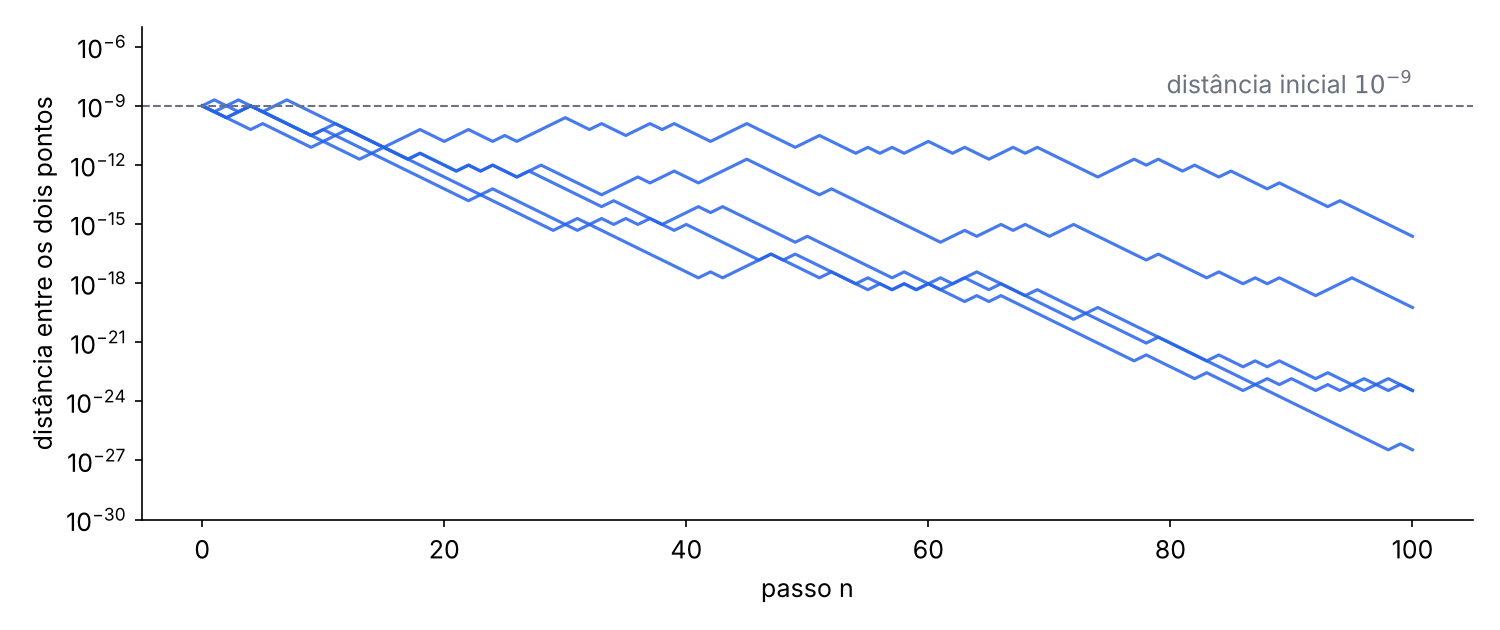
\includegraphics[width=0.49\linewidth]{figs/f2a_distancia_junta.png}\hfill
  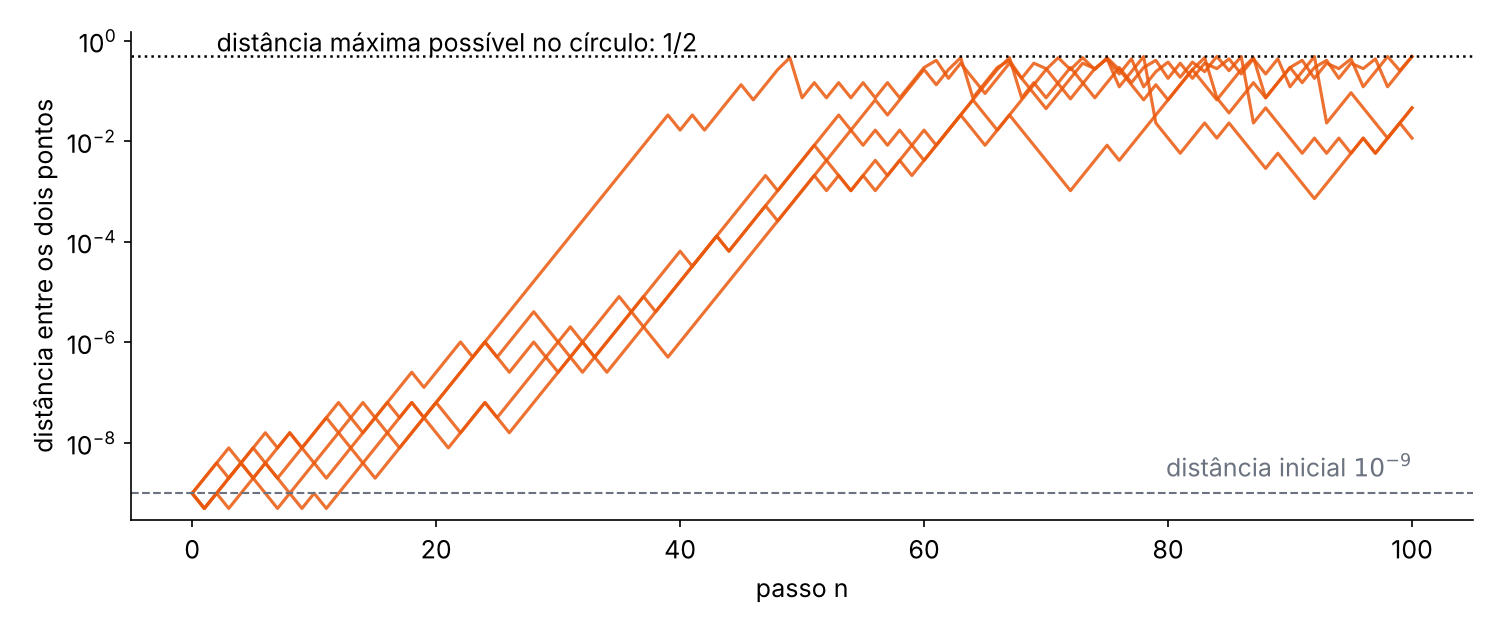
\includegraphics[width=0.49\linewidth]{figs/f2b_distancia_separa.png}
  \caption{Distância entre dois pontos inicialmente a $10^{-9}$, sob os mesmos sorteios
  (cada curva é uma sequência sorteada). Esquerda: $p=0{,}3$, os pontos se juntam.
  Direita: $p=0{,}7$, os pontos se separam até a distância máxima $\tfrac12$.}
  \label{fig:pelikan-dist}
\end{figure}

Essa é a intuição da entropia da fibra: ela mede quanta informação nova sobre $x_0$ é
preciso conhecer, a cada passo, para continuar prevendo a órbita. No regime que sincroniza,
nenhuma; no regime caótico, uma quantidade positiva.

% ---------------------------------------------------------------------
\subsection{O método de Ulam}
\label{subsec:pelikan-ulam}

Divida $[0,1)$ em $m$ células iguais $I_0,\dots,I_{m-1}$ e fixe uma palavra $\omega$ de tamanho
$n$. A \emph{matriz de Ulam} da palavra $\omega$ é
\[
  U^{(\omega)}_{ij}
  =\frac{\mathrm{Leb}\big(I_i\cap (f^n_\omega)^{-1}I_j\big)}{\mathrm{Leb}(I_i)}
  =\frac{\text{comprimento da parte de } I_i \text{ que cai em } I_j}{\text{comprimento de } I_i},
\]
ou seja, a fração da célula $i$ que termina na célula $j$ depois de aplicar os mapas de
$\omega$. Cada linha é uma distribuição de probabilidade, e sua entropia de Shannon
\[
  H_i(\omega)=-\sum_j U^{(\omega)}_{ij}\log U^{(\omega)}_{ij}
\]
mede o quanto a célula $i$ se espalhou: $H_i=0$ se ela cai inteira numa única célula e
$H_i=\log 2$ se ela se divide meio a meio entre duas. Definimos a média nas células e o
estimador de Ulam:
\[
  H(\omega)=\frac1m\sum_{i=0}^{m-1}H_i(\omega),\qquad
  \hat h_n(p)=\frac1n\sum_{\omega\in\{0,1\}^n}P_p(\omega)\,H(\omega).
\]
Note a ordem: calcula-se a entropia de cada palavra e só depois se faz a média sobre as
palavras (a sequência de sorteios é tratada como conhecida).

\begin{algorithm}[ht]
\caption{Estimador de Ulam para a entropia da fibra}
\begin{algorithmic}[1]
  \For{cada palavra $\omega$ de tamanho $n$}
    \For{cada célula $I_i$}
      \State espalhe muitos pontos dentro de $I_i$
      \State aplique os mapas de $\omega$, um por vez \Comment{0: $x/2$;\ 1: $2x\bmod 1$}
      \State $U_{ij}\gets$ fração dos pontos que terminaram em $I_j$
      \State $H_i\gets-\sum_j U_{ij}\log U_{ij}$
    \EndFor
    \State $H(\omega)\gets\frac1m\sum_i H_i$
  \EndFor
  \State \Return $\hat h_n=\frac1n\sum_\omega P_p(\omega)\,H(\omega)$
\end{algorithmic}
\end{algorithm}

Dois cuidados práticos: (i) usa-se a matriz da composição inteira $f^n_\omega$, e não o produto
de matrizes de um passo; (ii) a malha deve ser fina o bastante para $n$ passos ($m\ge 2^n$),
caso contrário a entropia de cada linha fica limitada por $\log m$ e $\hat h_n\to0$.

% ---------------------------------------------------------------------
\subsection{Exemplo com quatro células}
\label{subsec:pelikan-exemplo}

Tomemos $m=4$: $I_0=[0,\tfrac14)$, $I_1=[\tfrac14,\tfrac12)$, $I_2=[\tfrac12,\tfrac34)$,
$I_3=[\tfrac34,1)$.

\paragraph{Palavras de tamanho $n=1$.} A Tabela~\ref{tab:pelikan-n1} mostra para onde vai
cada célula. O ponto-chave é o \emph{tamanho} da imagem: $f_0$ reduz o tamanho pela metade, de
modo que a imagem ($\tfrac18$) cabe inteira numa célula; $f_1$ dobra o tamanho, de modo que a
imagem ($\tfrac12$) ocupa duas células, meio a meio.

\begin{table}[ht]
  \centering
  \small
  \begin{tabular}{cccc@{\qquad}cccc}
    \toprule
    \multicolumn{4}{c}{$f_0(x)=x/2$} & \multicolumn{4}{c}{$f_1(x)=2x\bmod 1$}\\
    \cmidrule(r){1-4}\cmidrule(l){5-8}
    célula & imagem & tam. & onde cai & célula & imagem & tam. & onde cai\\
    \midrule
    $I_0$ & $[0,\tfrac18)$ & $\tfrac18$ & $I_0$ &
    $I_0$ & $[0,\tfrac12)$ & $\tfrac12$ & $\tfrac12$ em $I_0$, $\tfrac12$ em $I_1$\\
    $I_1$ & $[\tfrac18,\tfrac14)$ & $\tfrac18$ & $I_0$ &
    $I_1$ & $[\tfrac12,1)$ & $\tfrac12$ & $\tfrac12$ em $I_2$, $\tfrac12$ em $I_3$\\
    $I_2$ & $[\tfrac14,\tfrac38)$ & $\tfrac18$ & $I_1$ &
    $I_2$ & $[0,\tfrac12)$ & $\tfrac12$ & $\tfrac12$ em $I_0$, $\tfrac12$ em $I_1$\\
    $I_3$ & $[\tfrac38,\tfrac12)$ & $\tfrac18$ & $I_1$ &
    $I_3$ & $[\tfrac12,1)$ & $\tfrac12$ & $\tfrac12$ em $I_2$, $\tfrac12$ em $I_3$\\
    \bottomrule
  \end{tabular}
  \caption{Imagens das quatro células por $f_0$ e $f_1$. Cada linha corresponde a uma linha da
  matriz de Ulam.}
  \label{tab:pelikan-n1}
\end{table}

As matrizes correspondentes são
\[
  U^{(0)}=\begin{pmatrix}1&0&0&0\\1&0&0&0\\0&1&0&0\\0&1&0&0\end{pmatrix},
  \qquad
  U^{(1)}=\begin{pmatrix}\tfrac12&\tfrac12&0&0\\0&0&\tfrac12&\tfrac12\\
  \tfrac12&\tfrac12&0&0\\0&0&\tfrac12&\tfrac12\end{pmatrix},
\]
com $H(0)=0$ e $H(1)=-2\cdot\tfrac12\log\tfrac12=\log2$. Logo
\[
  \hat h_1(p)=(1-p)\cdot 0+p\cdot\log2=p\log2 .
\]

\paragraph{Palavras de tamanho $n=2$.} Há quatro palavras:
\[
  \underbrace{\begin{pmatrix}1&0&0&0\\1&0&0&0\\1&0&0&0\\1&0&0&0\end{pmatrix}}_{\omega=00:\ x/4}
  \quad
  \underbrace{\begin{pmatrix}1&0&0&0\\0&1&0&0\\0&0&1&0\\0&0&0&1\end{pmatrix}}_{\omega=01:\ x}
  \quad
  \underbrace{\begin{pmatrix}1&0&0&0\\0&1&0&0\\1&0&0&0\\0&1&0&0\end{pmatrix}}_{\omega=10:\ \frac12(2x\bmod1)}
  \quad
  \underbrace{\begin{pmatrix}\tfrac14&\tfrac14&\tfrac14&\tfrac14\\\tfrac14&\tfrac14&\tfrac14&\tfrac14\\
  \tfrac14&\tfrac14&\tfrac14&\tfrac14\\\tfrac14&\tfrac14&\tfrac14&\tfrac14\end{pmatrix}}_{\omega=11:\ 4x\bmod1}
\]
com entropias $0$, $0$, $0$ e $\log4$, e probabilidades $(1-p)^2$, $(1-p)p$, $p(1-p)$ e $p^2$.
Portanto
\[
  \hat h_2(p)=\frac12\Big[(1-p)^2\cdot0+2p(1-p)\cdot0+p^2\cdot\log4\Big]=p^2\log2 .
\]
Repare que nas palavras $01$ e $10$ uma contração desfaz uma expansão, e nada se espalha. É por
isso que $\hat h_2<\hat h_1$: a média ingênua $p\log 2$ superestima a entropia.

% ---------------------------------------------------------------------
\subsection{Generalização: só o saldo positivo conta}
\label{subsec:pelikan-geral}

Numa palavra com $N_1(\omega)=j$ uns e $N_0(\omega)=n-j$ zeros, o mapa $f^n_\omega$ tem
inclinação $2^{S(\omega)}$ em cada célula, onde
\[
  S(\omega)=N_1(\omega)-N_0(\omega)=2j-n .
\]
A ordem dos mapas não altera o tamanho da imagem, só a contagem. Assim:
\begin{itemize}
  \item se $S(\omega)>0$, cada célula se espalha igualmente por $2^{S(\omega)}$ células, e
        $H(\omega)=-\sum 2^{-S}\log2^{-S}=S(\omega)\log 2$;
  \item se $S(\omega)\le0$, cada célula cai dentro de uma só, e $H(\omega)=0$.
\end{itemize}
Isto é, $H(\omega)=S(\omega)^+\log2$, onde $a^+=\max\{a,0\}$. Agrupando as palavras pelo número
$j$ de uns,
\[
  \hat h_n(p)=\frac1n\sum_\omega P_p(\omega)\,S(\omega)^+\log2
  =\frac{\log2}{n}\sum_{j=0}^{n}\binom nj p^j(1-p)^{n-j}\,(2j-n)^+ .
\]

\paragraph{O limite.} Se $J\sim\mathrm{Binomial}(n,p)$ é o número de uns de uma palavra
sorteada, a fórmula acima é
\[
  \hat h_n(p)=\log2\;\mathbb E\Big[\big(2\tfrac Jn-1\big)^+\Big].
\]
Pela lei dos grandes números, $J/n\to p$; como $t\mapsto(2t-1)^+$ é contínua e limitada em
$[0,1]$, obtemos
\[
  \hat h_n(p)\xrightarrow[n\to\infty]{}(2p-1)^+\log2 .
\]
Perto de $p=\tfrac12$ a convergência é lenta: $J/n$ oscila em torno de $\tfrac12$ com desvio da
ordem de $1/\sqrt n$, e a parte positiva ``aproveita'' as oscilações para cima, de modo que o
erro só decai como $1/\sqrt n$.

\paragraph{Observação.} Neste exemplo ``controlado'' há fórmula fechada e o limite coincide com
a entropia exata da fibra, $h_{\mathrm{fib}}(p)=(2p-1)^+\log2$, que pode ser obtida diretamente
pela definição contando quantos dígitos binários de $x_0$ a dinâmica revela por passo. Em
sistemas gerais não há tal fórmula, e o cálculo numérico de $\hat h_n$ é o caminho disponível.

% ---------------------------------------------------------------------
\subsection{Resultados numéricos}
\label{subsec:pelikan-resultados}

A Figura~\ref{fig:pelikan-principal} mostra $\hat h_n(p)$ para vários comprimentos de palavra.
Para $n=1$ obtemos a reta $p\log2$; conforme $n$ cresce, as curvas se aproximam de
$(2p-1)^+\log2$, que é nula até $p=\tfrac12$.

\begin{figure}[ht]
  \centering
  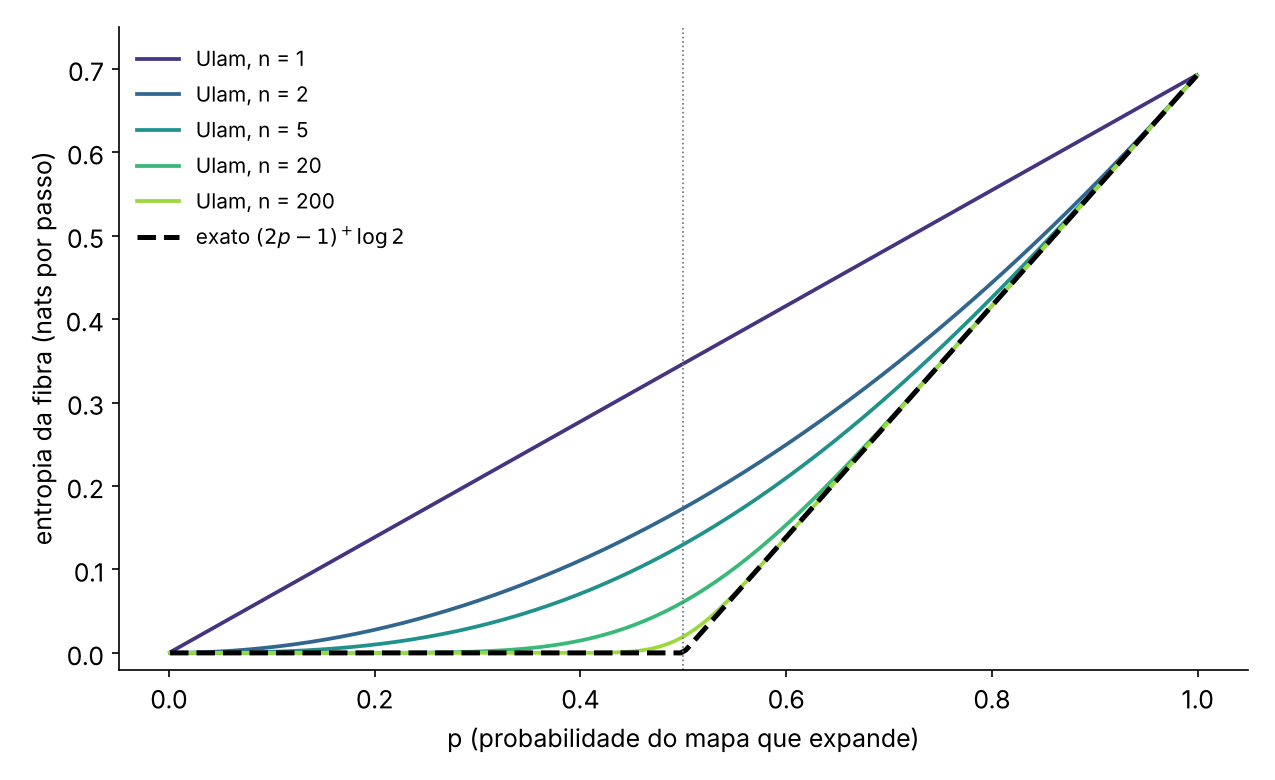
\includegraphics[width=0.72\linewidth]{figs/f7_principal.png}
  \caption{Estimador de Ulam $\hat h_n(p)$ para $n=1,2,5,20,200$ e valor exato
  $(2p-1)^+\log2$ (tracejado).}
  \label{fig:pelikan-principal}
\end{figure}

A Figura~\ref{fig:pelikan-conv} mostra a convergência em $n$ para valores fixos de $p$: longe
de $p=\tfrac12$ poucos passos bastam; em $p=\tfrac12$ a aproximação é a mais lenta.

\begin{figure}[ht]
  \centering
  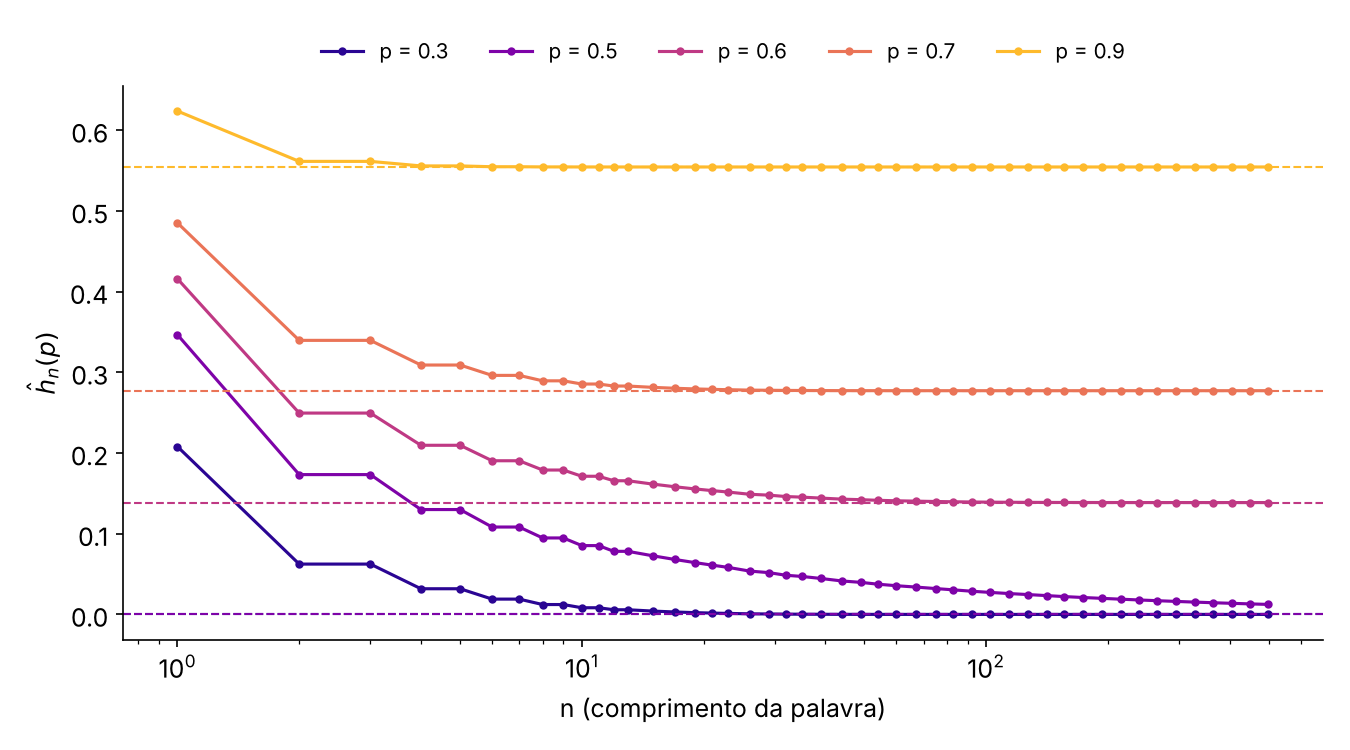
\includegraphics[width=0.75\linewidth]{figs/f9_convergencia_p.png}
  \caption{$\hat h_n(p)$ em função de $n$ para $p=0{,}3;\,0{,}5;\,0{,}6;\,0{,}7;\,0{,}9$. As linhas
  tracejadas são os valores exatos.}
  \label{fig:pelikan-conv}
\end{figure}

\paragraph{Como as curvas foram calculadas.} Para $n$ pequeno, as matrizes de Ulam foram
construídas diretamente (espalhando pontos em cada célula e aplicando os mapas). Para $n$
grande isso é inviável, pois há $2^n$ palavras; usamos então a fórmula fechada da
Seção~\ref{subsec:pelikan-geral}, que fornece \emph{exatamente} o mesmo valor que as matrizes.
A Tabela~\ref{tab:pelikan-conf} mostra a concordância para $n=4$.

\begin{table}[ht]
  \centering
  \begin{tabular}{ccc}
    \toprule
    $p$ & matrizes de Ulam ($n=4$) & fórmula fechada ($n=4$)\\
    \midrule
    0,3 & 0,03182 & 0,03182\\
    0,7 & 0,30907 & 0,30907\\
    0,9 & 0,55583 & 0,55583\\
    \bottomrule
  \end{tabular}
  \caption{Conferência entre as matrizes de Ulam construídas numericamente e a fórmula fechada.}
  \label{tab:pelikan-conf}
\end{table}

Por exemplo, para $p=0{,}7$: $\hat h_1=0{,}485$, $\hat h_2=0{,}340$, $\hat h_5=0{,}309$,
$\hat h_{20}=0{,}279$ e $\hat h_{200}=0{,}2773$, que já coincide com $0{,}4\log2\approx0{,}2773$.

% ---------------------------------------------------------------------
\subsection{Conclusões}

\begin{enumerate}
  \item \textbf{Precisão finita.} Em \texttt{double}, as órbitas deste sistema morrem em cerca de
        $53/(2p-1)$ passos; mais precisão só adia o problema. Métodos que dependem de órbitas
        longas não são confiáveis aqui.
  \item \textbf{Dois regimes.} Os mesmos dois mapas geram comportamentos opostos: para
        $p<\tfrac12$ as órbitas sincronizam, para $p>\tfrac12$ há dependência sensível. O que
        decide é o saldo entre expansões e contrações.
  \item \textbf{Método de Ulam.} O estimador mede o quanto as células se espalham usando poucos
        passos, e converge para $h_{\mathrm{fib}}(p)=(2p-1)^+\log2$, lentamente perto de
        $p=\tfrac12$. A média ingênua $p\log2$ está errada.
\end{enumerate}

% ---------------------------------------------------------------------
\subsection{Material complementar}

O repositório \url{\repoPelikan} contém:
\begin{itemize}
  \item o \emph{notebook} Jupyter que gera todas as figuras desta seção, com o código comentado e
        uma célula para experimentar outros valores de $p$ e $n$;
  \item os slides da apresentação (fonte \LaTeX{} e PDF).
\end{itemize}

\paragraph{Referências.}
\begin{itemize}
  \item Nota \emph{Ulam entropy} (material do curso), que contém a demonstração de que
        $h_{\mathrm{fib}}(p)=(2p-1)^+\log2$ e da fórmula fechada para $\hat h_n$.
  \item G.~Froyland, \emph{Ulam's method for random interval maps}, Nonlinearity \textbf{12}
        (1999), 1029--1052.
  \item C.~Monthus, \emph{Explicit dynamical properties of the Pelikan random map in the chaotic
        region and at the intermittent critical point towards the non-chaotic region},
        J.~Stat.~Mech.\ (2025), 013212.
  \item G.~Froyland, O.~Junge, G.~Ochs, \emph{Rigorous computation of topological entropy with
        respect to a finite partition}, Physica D \textbf{154} (2001), 68--84.
\end{itemize}

%  Pacotes necessários no preâmbulo da apostila:
%    amsmath, amssymb, graphicx, booktabs, hyperref, algorithm, algpseudocode
%  As figuras ficam na pasta figs/ (geradas pelo notebook do repositório).
%
\providecommand{\repoPelikan}{https://github.com/EdeilsonAzevedo/seminario-entropia-ulam}
% =====================================================================

\section{Entropia da fibra de um sistema aleatório: cálculo numérico pelo método de Ulam}
\label{sec:pelikan}

Nesta seção estudamos, de forma essencialmente numérica, a entropia da fibra de um
sistema aleatório muito simples, formado por dois mapas do intervalo: um que contrai e
outro que expande. O objetivo é mostrar como o \emph{método de Ulam} permite calcular essa
entropia e entender como ela depende da probabilidade de sortear cada mapa. Por ser um
exemplo ``controlado'', o valor exato é conhecido, o que permite validar a simulação.

Todo o código (um \emph{notebook} Jupyter que gera as figuras desta seção) e os slides da
apresentação estão disponíveis em
\begin{center}
  \url{\repoPelikan}
\end{center}

% ---------------------------------------------------------------------
\subsection{O sistema}
\label{subsec:pelikan-sistema}

\paragraph{Base.} A base é o \emph{shift} sobre as sequências de 0s e 1s:
\[
  \Omega=\{0,1\}^{\mathbb N},\qquad
  \sigma(\omega_0\omega_1\omega_2\ldots)=\omega_1\omega_2\ldots
\]
Cada símbolo é sorteado de forma independente: $\omega_k=1$ com probabilidade $p$ e
$\omega_k=0$ com probabilidade $1-p$.

\paragraph{Fibra.} A fibra é o intervalo $[0,1)$, onde agem dois mapas:
\[
  f_0(x)=\frac{x}{2}\quad\text{(contrai)},\qquad
  f_1(x)=2x \bmod 1\quad\text{(expande)}.
\]

\paragraph{Produto torcido.} O sistema completo é
\[
  F:\Omega\times[0,1)\to\Omega\times[0,1),\qquad
  F(\omega,x)=\big(\sigma\omega,\ f_{\omega_0}(x)\big).
\]
A base anda sozinha; a fibra ``obedece'' ao símbolo lido na base. Iterando,
\[
  F^n(\omega,x)=\big(\sigma^n\omega,\ f^n_\omega(x)\big),\qquad
  f^n_\omega=f_{\omega_{n-1}}\circ\cdots\circ f_{\omega_1}\circ f_{\omega_0},
\]
isto é, a cada passo o shift traz o próximo símbolo para a posição $0$, e é ele que escolhe
o mapa aplicado.

\paragraph{Notação para palavras.} Uma \emph{palavra} de tamanho $n$ é
$\omega=\omega_0\cdots\omega_{n-1}\in\{0,1\}^n$. Escrevemos
\[
  N_1(\omega)=\text{nº de 1s},\qquad N_0(\omega)=\text{nº de 0s},\qquad
  P_p(\omega)=p^{N_1(\omega)}(1-p)^{N_0(\omega)},
\]
de modo que $P_p(\omega)$ é a probabilidade de sortear a palavra $\omega$.

\paragraph{Leitura em binário.} Se $x=0{,}b_1b_2b_3\ldots$ em base 2, então
\[
  f_0(x)=0{,}0\,b_1b_2\ldots \quad\text{(insere um 0 na frente)},\qquad
  f_1(x)=0{,}b_2b_3\ldots \quad\text{(apaga o primeiro dígito)}.
\]
Essa observação simples explica quase todos os fenômenos desta seção.

\paragraph{Objetivo.} Calcular numericamente a entropia da fibra, $h_{\mathrm{fib}}(p)$,
pelo método de Ulam, e entender como ela depende de $p$.

% ---------------------------------------------------------------------
\subsection{Um alerta numérico: precisão finita}
\label{subsec:pelikan-precisao}

Antes de simular, convém notar um problema que \emph{não} é do sistema, mas do computador.
Um número em ponto flutuante de precisão dupla (\texttt{double}) guarda 53 dígitos
binários. Como $f_1$ apaga o primeiro dígito, depois de 53 aplicações de $2x\bmod1$ não
sobra dígito algum: a órbita vira exatamente $0$ e fica presa ali para sempre
(Figura~\ref{fig:pelikan-float}, à esquerda). A órbita verdadeira, calculada com
aritmética exata, continua normalmente.

\begin{figure}[ht]
  \centering
  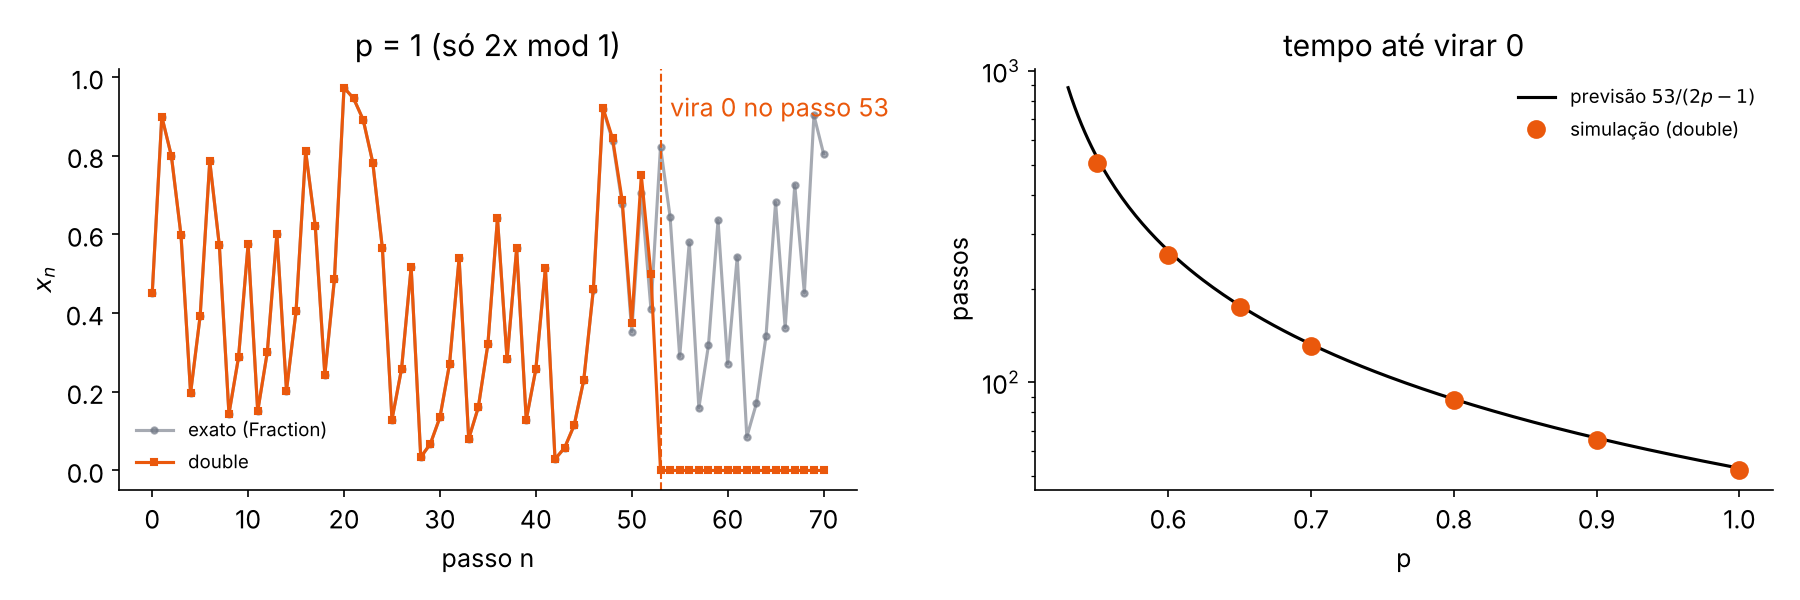
\includegraphics[width=\linewidth]{figs/f3_float.png}
  \caption{Esquerda: com $p=1$ (só $2x\bmod 1$) a órbita em \texttt{double} vira $0$ no passo 53,
  enquanto a órbita exata continua. Direita: tempo médio até a órbita em \texttt{double}
  virar $0$, comparado com a previsão $53/(2p-1)$.}
  \label{fig:pelikan-float}
\end{figure}

\paragraph{Por que $53/(2p-1)$.} Com probabilidade $p$ sai $f_1$, que consome um dígito; com
probabilidade $1-p$ sai $f_0$, que apenas insere um zero, que será apagado ``de graça''
depois. Em média, cada passo consome
\[
  p\cdot(+1)+(1-p)\cdot(-1)=2p-1
\]
dígitos. Com 53 dígitos disponíveis, a órbita dura cerca de $53/(2p-1)$ passos
(Figura~\ref{fig:pelikan-float}, à direita). Por exemplo, para $p=0{,}7$ a previsão é
de $132$ passos, e a média medida foi $129$.

\paragraph{Mais precisão só adia.} Bibliotecas de precisão arbitrária
(\texttt{mpmath}, \texttt{Fraction}) aumentam o número de bits, mas não eliminam o problema:
com $B$ bits a órbita dura $\approx B/(2p-1)$ passos. Inversamente, para simular $T$ passos
são necessários $\approx(2p-1)\,T$ bits, que crescem sem limite
(Figura~\ref{fig:pelikan-precisao}). Com $p=0{,}7$, medimos tempos de vida de
$129$, $282$, $623$ e $1232$ passos para $53$, $113$, $250$ e $500$ bits, respectivamente.

\begin{figure}[ht]
  \centering
  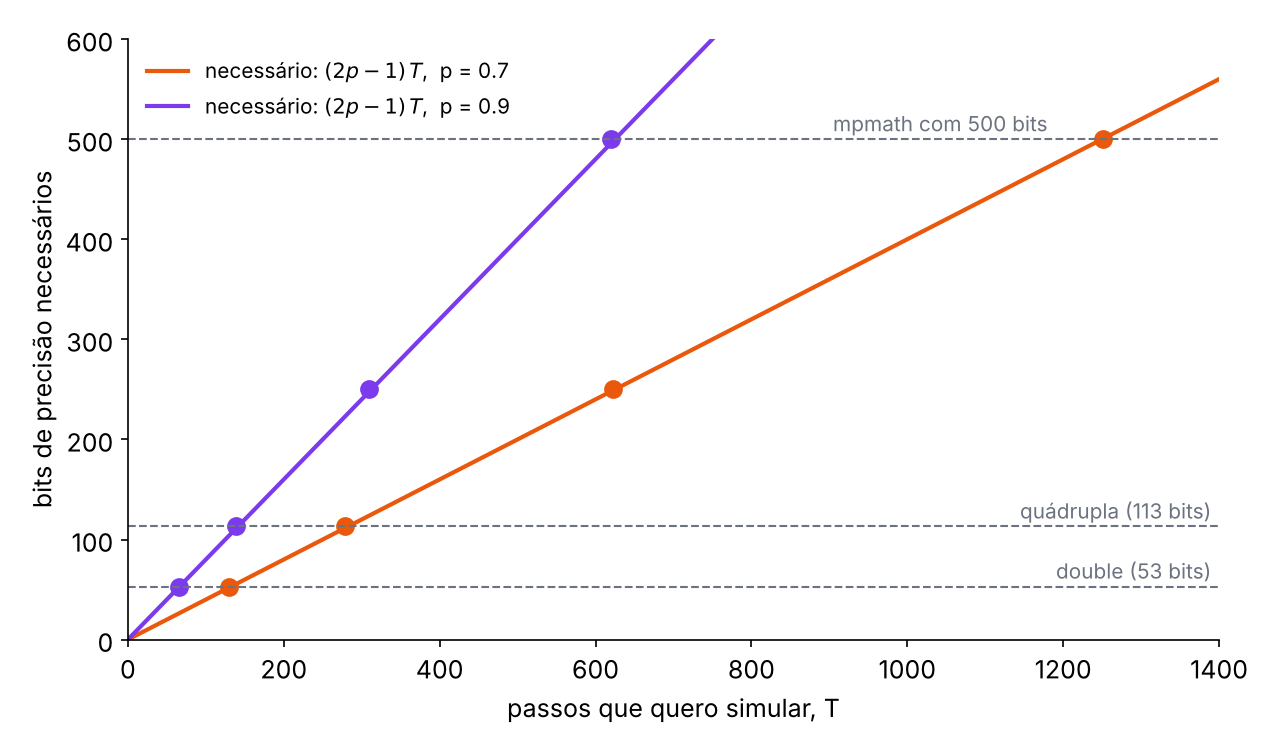
\includegraphics[width=0.7\linewidth]{figs/f3b_precisao.png}
  \caption{Bits necessários para simular $T$ passos: retas $(2p-1)\,T$ e pontos medidos com
  \texttt{mpmath}. Toda precisão fixa (linhas tracejadas) acaba sendo ultrapassada.}
  \label{fig:pelikan-precisao}
\end{figure}

\paragraph{Consequência.} Um método que precise seguir órbitas longas para estimar a entropia
não é confiável neste sistema. Precisamos de um método que use \emph{poucos passos} de cada
vez, e é isso que o método de Ulam oferece. Nas figuras de órbitas a seguir, usamos
aritmética exata.

% ---------------------------------------------------------------------
\subsection{O que sabemos e o que queremos saber}

Os casos extremos são simples:
\begin{itemize}
  \item $p=1$: só $2x\bmod1$, e a entropia da fibra é $\log 2$;
  \item $p=0$: só contração, e a entropia da fibra é $0$.
\end{itemize}
As perguntas são: o que acontece para $0<p<1$? A resposta é a média ingênua $p\log 2$?
O método de Ulam calcula $h_{\mathrm{fib}}$, e com que velocidade converge?

% ---------------------------------------------------------------------
\subsection{Comportamento das órbitas}

A Figura~\ref{fig:pelikan-traj} mostra uma órbita típica para dois valores de $p$. Com
$p=0{,}3$ a órbita cola em $0$; com $p=0{,}7$ ela percorre o intervalo todo.

\begin{figure}[ht]
  \centering
  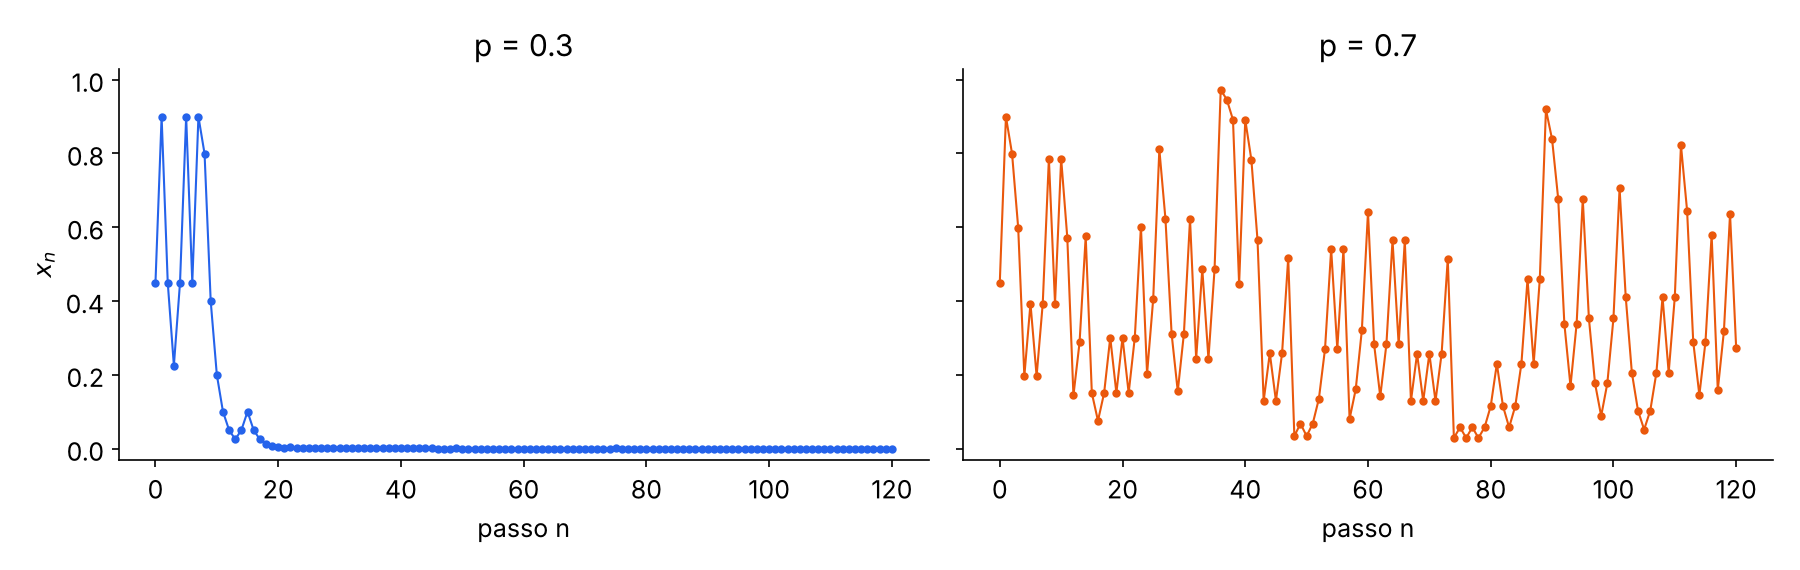
\includegraphics[width=\linewidth]{figs/f1_trajetorias.png}
  \caption{Uma órbita $x_n$ para $p=0{,}3$ (esquerda) e $p=0{,}7$ (direita).}
  \label{fig:pelikan-traj}
\end{figure}

Para entender a diferença, tomamos dois pontos quase iguais, $x_0$ e $y_0=x_0+10^{-9}$, e
aplicamos \emph{a mesma} sequência de mapas aos dois. Cada $f_1$ dobra a distância e cada
$f_0$ a divide por 2, de modo que
\[
  |x_n-y_n|\approx 2^{S_n}\,|x_0-y_0|,\qquad S_n=N_1-N_0 \text{ nos $n$ primeiros sorteios}.
\]
Com $p<\tfrac12$ as contrações vencem e os pontos se juntam: o sistema \emph{esquece} a
condição inicial (sincronização). Com $p>\tfrac12$ as expansões vencem e um erro de $10^{-9}$
cresce até o tamanho do intervalo (dependência sensível às condições iniciais). No
círculo $[0,1)$ a distância nunca passa de $\tfrac12$, por isso as curvas saturam nesse valor
(Figura~\ref{fig:pelikan-dist}).

\begin{figure}[ht]
  \centering
  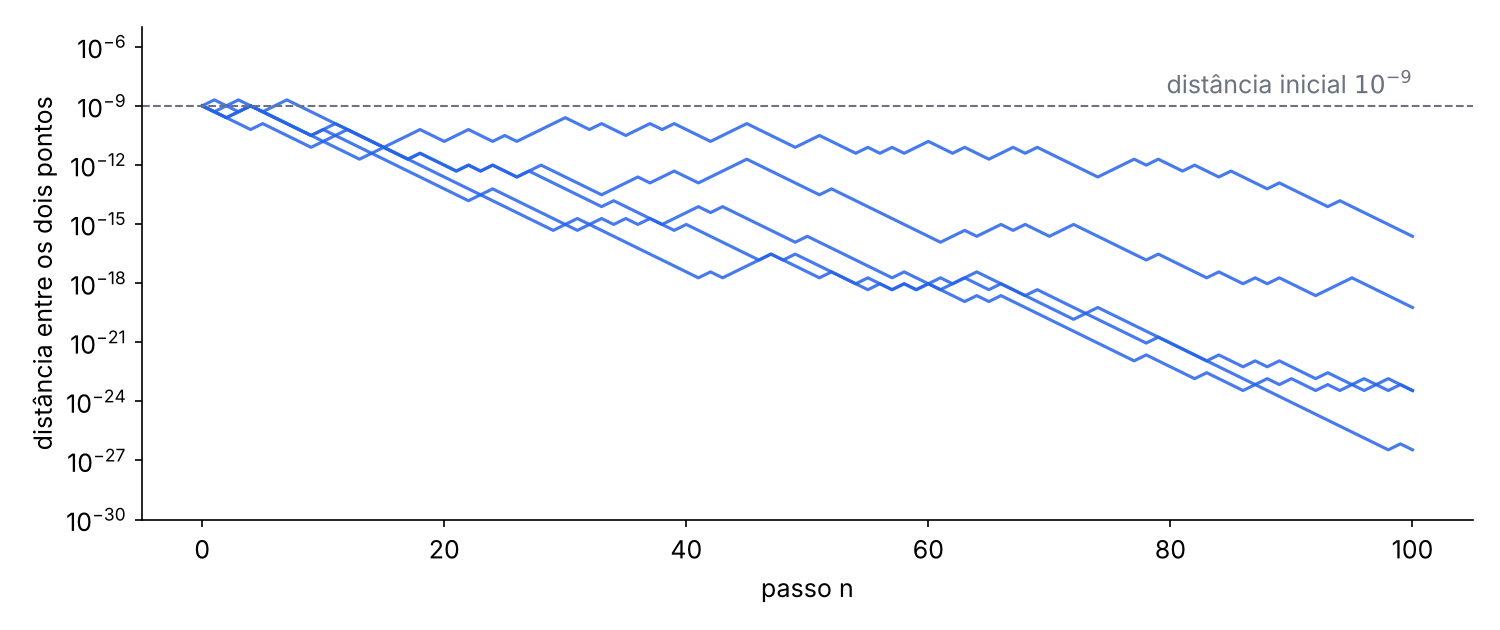
\includegraphics[width=0.49\linewidth]{figs/f2a_distancia_junta.png}\hfill
  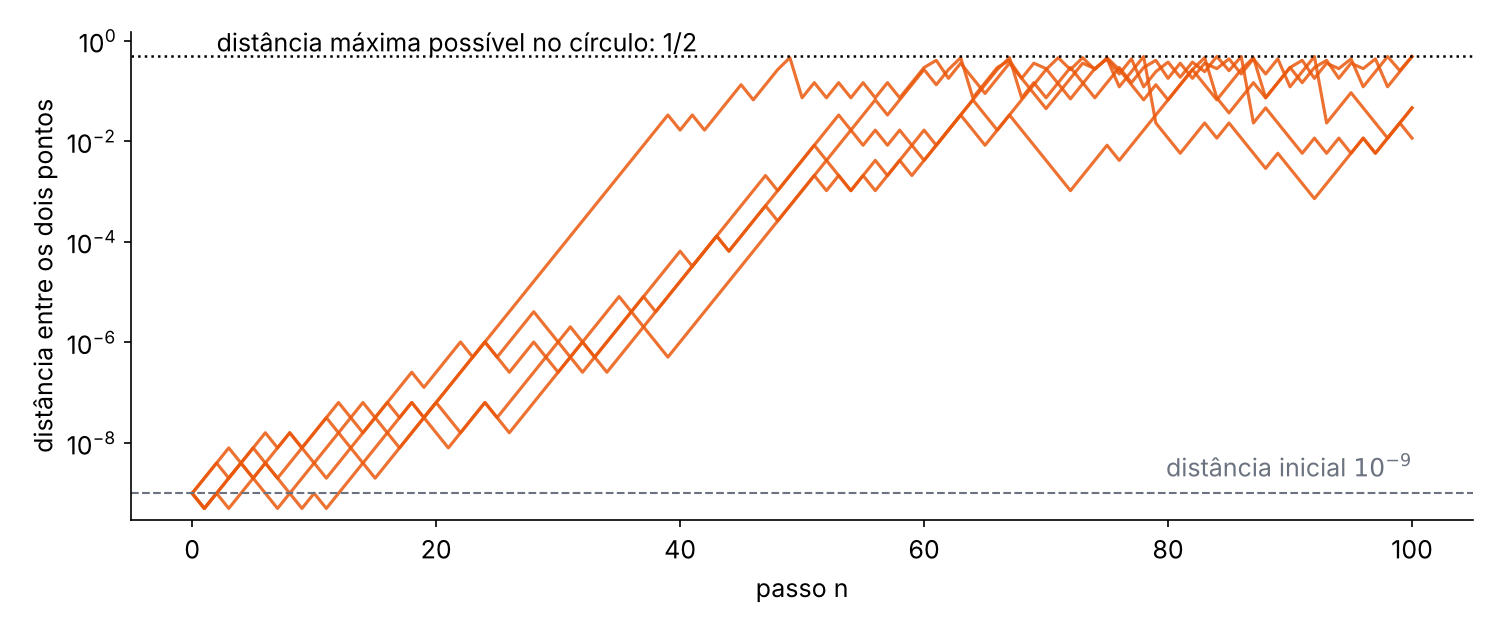
\includegraphics[width=0.49\linewidth]{figs/f2b_distancia_separa.png}
  \caption{Distância entre dois pontos inicialmente a $10^{-9}$, sob os mesmos sorteios
  (cada curva é uma sequência sorteada). Esquerda: $p=0{,}3$, os pontos se juntam.
  Direita: $p=0{,}7$, os pontos se separam até a distância máxima $\tfrac12$.}
  \label{fig:pelikan-dist}
\end{figure}

Essa é a intuição da entropia da fibra: ela mede quanta informação nova sobre $x_0$ é
preciso conhecer, a cada passo, para continuar prevendo a órbita. No regime que sincroniza,
nenhuma; no regime caótico, uma quantidade positiva.

% ---------------------------------------------------------------------
\subsection{O método de Ulam}
\label{subsec:pelikan-ulam}

Divida $[0,1)$ em $m$ células iguais $I_0,\dots,I_{m-1}$ e fixe uma palavra $\omega$ de tamanho
$n$. A \emph{matriz de Ulam} da palavra $\omega$ é
\[
  U^{(\omega)}_{ij}
  =\frac{\mathrm{Leb}\big(I_i\cap (f^n_\omega)^{-1}I_j\big)}{\mathrm{Leb}(I_i)}
  =\frac{\text{comprimento da parte de } I_i \text{ que cai em } I_j}{\text{comprimento de } I_i},
\]
ou seja, a fração da célula $i$ que termina na célula $j$ depois de aplicar os mapas de
$\omega$. Cada linha é uma distribuição de probabilidade, e sua entropia de Shannon
\[
  H_i(\omega)=-\sum_j U^{(\omega)}_{ij}\log U^{(\omega)}_{ij}
\]
mede o quanto a célula $i$ se espalhou: $H_i=0$ se ela cai inteira numa única célula e
$H_i=\log 2$ se ela se divide meio a meio entre duas. Definimos a média nas células e o
estimador de Ulam:
\[
  H(\omega)=\frac1m\sum_{i=0}^{m-1}H_i(\omega),\qquad
  \hat h_n(p)=\frac1n\sum_{\omega\in\{0,1\}^n}P_p(\omega)\,H(\omega).
\]
Note a ordem: calcula-se a entropia de cada palavra e só depois se faz a média sobre as
palavras (a sequência de sorteios é tratada como conhecida).

\begin{algorithm}[ht]
\caption{Estimador de Ulam para a entropia da fibra}
\begin{algorithmic}[1]
  \For{cada palavra $\omega$ de tamanho $n$}
    \For{cada célula $I_i$}
      \State espalhe muitos pontos dentro de $I_i$
      \State aplique os mapas de $\omega$, um por vez \Comment{0: $x/2$;\ 1: $2x\bmod 1$}
      \State $U_{ij}\gets$ fração dos pontos que terminaram em $I_j$
      \State $H_i\gets-\sum_j U_{ij}\log U_{ij}$
    \EndFor
    \State $H(\omega)\gets\frac1m\sum_i H_i$
  \EndFor
  \State \Return $\hat h_n=\frac1n\sum_\omega P_p(\omega)\,H(\omega)$
\end{algorithmic}
\end{algorithm}

Dois cuidados práticos: (i) usa-se a matriz da composição inteira $f^n_\omega$, e não o produto
de matrizes de um passo; (ii) a malha deve ser fina o bastante para $n$ passos ($m\ge 2^n$),
caso contrário a entropia de cada linha fica limitada por $\log m$ e $\hat h_n\to0$.

% ---------------------------------------------------------------------
\subsection{Exemplo com quatro células}
\label{subsec:pelikan-exemplo}

Tomemos $m=4$: $I_0=[0,\tfrac14)$, $I_1=[\tfrac14,\tfrac12)$, $I_2=[\tfrac12,\tfrac34)$,
$I_3=[\tfrac34,1)$.

\paragraph{Palavras de tamanho $n=1$.} A Tabela~\ref{tab:pelikan-n1} mostra para onde vai
cada célula. O ponto-chave é o \emph{tamanho} da imagem: $f_0$ reduz o tamanho pela metade, de
modo que a imagem ($\tfrac18$) cabe inteira numa célula; $f_1$ dobra o tamanho, de modo que a
imagem ($\tfrac12$) ocupa duas células, meio a meio.

\begin{table}[ht]
  \centering
  \small
  \begin{tabular}{cccc@{\qquad}cccc}
    \toprule
    \multicolumn{4}{c}{$f_0(x)=x/2$} & \multicolumn{4}{c}{$f_1(x)=2x\bmod 1$}\\
    \cmidrule(r){1-4}\cmidrule(l){5-8}
    célula & imagem & tam. & onde cai & célula & imagem & tam. & onde cai\\
    \midrule
    $I_0$ & $[0,\tfrac18)$ & $\tfrac18$ & $I_0$ &
    $I_0$ & $[0,\tfrac12)$ & $\tfrac12$ & $\tfrac12$ em $I_0$, $\tfrac12$ em $I_1$\\
    $I_1$ & $[\tfrac18,\tfrac14)$ & $\tfrac18$ & $I_0$ &
    $I_1$ & $[\tfrac12,1)$ & $\tfrac12$ & $\tfrac12$ em $I_2$, $\tfrac12$ em $I_3$\\
    $I_2$ & $[\tfrac14,\tfrac38)$ & $\tfrac18$ & $I_1$ &
    $I_2$ & $[0,\tfrac12)$ & $\tfrac12$ & $\tfrac12$ em $I_0$, $\tfrac12$ em $I_1$\\
    $I_3$ & $[\tfrac38,\tfrac12)$ & $\tfrac18$ & $I_1$ &
    $I_3$ & $[\tfrac12,1)$ & $\tfrac12$ & $\tfrac12$ em $I_2$, $\tfrac12$ em $I_3$\\
    \bottomrule
  \end{tabular}
  \caption{Imagens das quatro células por $f_0$ e $f_1$. Cada linha corresponde a uma linha da
  matriz de Ulam.}
  \label{tab:pelikan-n1}
\end{table}

As matrizes correspondentes são
\[
  U^{(0)}=\begin{pmatrix}1&0&0&0\\1&0&0&0\\0&1&0&0\\0&1&0&0\end{pmatrix},
  \qquad
  U^{(1)}=\begin{pmatrix}\tfrac12&\tfrac12&0&0\\0&0&\tfrac12&\tfrac12\\
  \tfrac12&\tfrac12&0&0\\0&0&\tfrac12&\tfrac12\end{pmatrix},
\]
com $H(0)=0$ e $H(1)=-2\cdot\tfrac12\log\tfrac12=\log2$. Logo
\[
  \hat h_1(p)=(1-p)\cdot 0+p\cdot\log2=p\log2 .
\]

\paragraph{Palavras de tamanho $n=2$.} Há quatro palavras:
\[
  \underbrace{\begin{pmatrix}1&0&0&0\\1&0&0&0\\1&0&0&0\\1&0&0&0\end{pmatrix}}_{\omega=00:\ x/4}
  \quad
  \underbrace{\begin{pmatrix}1&0&0&0\\0&1&0&0\\0&0&1&0\\0&0&0&1\end{pmatrix}}_{\omega=01:\ x}
  \quad
  \underbrace{\begin{pmatrix}1&0&0&0\\0&1&0&0\\1&0&0&0\\0&1&0&0\end{pmatrix}}_{\omega=10:\ \frac12(2x\bmod1)}
  \quad
  \underbrace{\begin{pmatrix}\tfrac14&\tfrac14&\tfrac14&\tfrac14\\\tfrac14&\tfrac14&\tfrac14&\tfrac14\\
  \tfrac14&\tfrac14&\tfrac14&\tfrac14\\\tfrac14&\tfrac14&\tfrac14&\tfrac14\end{pmatrix}}_{\omega=11:\ 4x\bmod1}
\]
com entropias $0$, $0$, $0$ e $\log4$, e probabilidades $(1-p)^2$, $(1-p)p$, $p(1-p)$ e $p^2$.
Portanto
\[
  \hat h_2(p)=\frac12\Big[(1-p)^2\cdot0+2p(1-p)\cdot0+p^2\cdot\log4\Big]=p^2\log2 .
\]
Repare que nas palavras $01$ e $10$ uma contração desfaz uma expansão, e nada se espalha. É por
isso que $\hat h_2<\hat h_1$: a média ingênua $p\log 2$ superestima a entropia.

% ---------------------------------------------------------------------
\subsection{Generalização: só o saldo positivo conta}
\label{subsec:pelikan-geral}

Numa palavra com $N_1(\omega)=j$ uns e $N_0(\omega)=n-j$ zeros, o mapa $f^n_\omega$ tem
inclinação $2^{S(\omega)}$ em cada célula, onde
\[
  S(\omega)=N_1(\omega)-N_0(\omega)=2j-n .
\]
A ordem dos mapas não altera o tamanho da imagem, só a contagem. Assim:
\begin{itemize}
  \item se $S(\omega)>0$, cada célula se espalha igualmente por $2^{S(\omega)}$ células, e
        $H(\omega)=-\sum 2^{-S}\log2^{-S}=S(\omega)\log 2$;
  \item se $S(\omega)\le0$, cada célula cai dentro de uma só, e $H(\omega)=0$.
\end{itemize}
Isto é, $H(\omega)=S(\omega)^+\log2$, onde $a^+=\max\{a,0\}$. Agrupando as palavras pelo número
$j$ de uns,
\[
  \hat h_n(p)=\frac1n\sum_\omega P_p(\omega)\,S(\omega)^+\log2
  =\frac{\log2}{n}\sum_{j=0}^{n}\binom nj p^j(1-p)^{n-j}\,(2j-n)^+ .
\]

\paragraph{O limite.} Se $J\sim\mathrm{Binomial}(n,p)$ é o número de uns de uma palavra
sorteada, a fórmula acima é
\[
  \hat h_n(p)=\log2\;\mathbb E\Big[\big(2\tfrac Jn-1\big)^+\Big].
\]
Pela lei dos grandes números, $J/n\to p$; como $t\mapsto(2t-1)^+$ é contínua e limitada em
$[0,1]$, obtemos
\[
  \hat h_n(p)\xrightarrow[n\to\infty]{}(2p-1)^+\log2 .
\]
Perto de $p=\tfrac12$ a convergência é lenta: $J/n$ oscila em torno de $\tfrac12$ com desvio da
ordem de $1/\sqrt n$, e a parte positiva ``aproveita'' as oscilações para cima, de modo que o
erro só decai como $1/\sqrt n$.

\paragraph{Observação.} Neste exemplo ``controlado'' há fórmula fechada e o limite coincide com
a entropia exata da fibra, $h_{\mathrm{fib}}(p)=(2p-1)^+\log2$, que pode ser obtida diretamente
pela definição contando quantos dígitos binários de $x_0$ a dinâmica revela por passo. Em
sistemas gerais não há tal fórmula, e o cálculo numérico de $\hat h_n$ é o caminho disponível.

% ---------------------------------------------------------------------
\subsection{Resultados numéricos}
\label{subsec:pelikan-resultados}

A Figura~\ref{fig:pelikan-principal} mostra $\hat h_n(p)$ para vários comprimentos de palavra.
Para $n=1$ obtemos a reta $p\log2$; conforme $n$ cresce, as curvas se aproximam de
$(2p-1)^+\log2$, que é nula até $p=\tfrac12$.

\begin{figure}[ht]
  \centering
  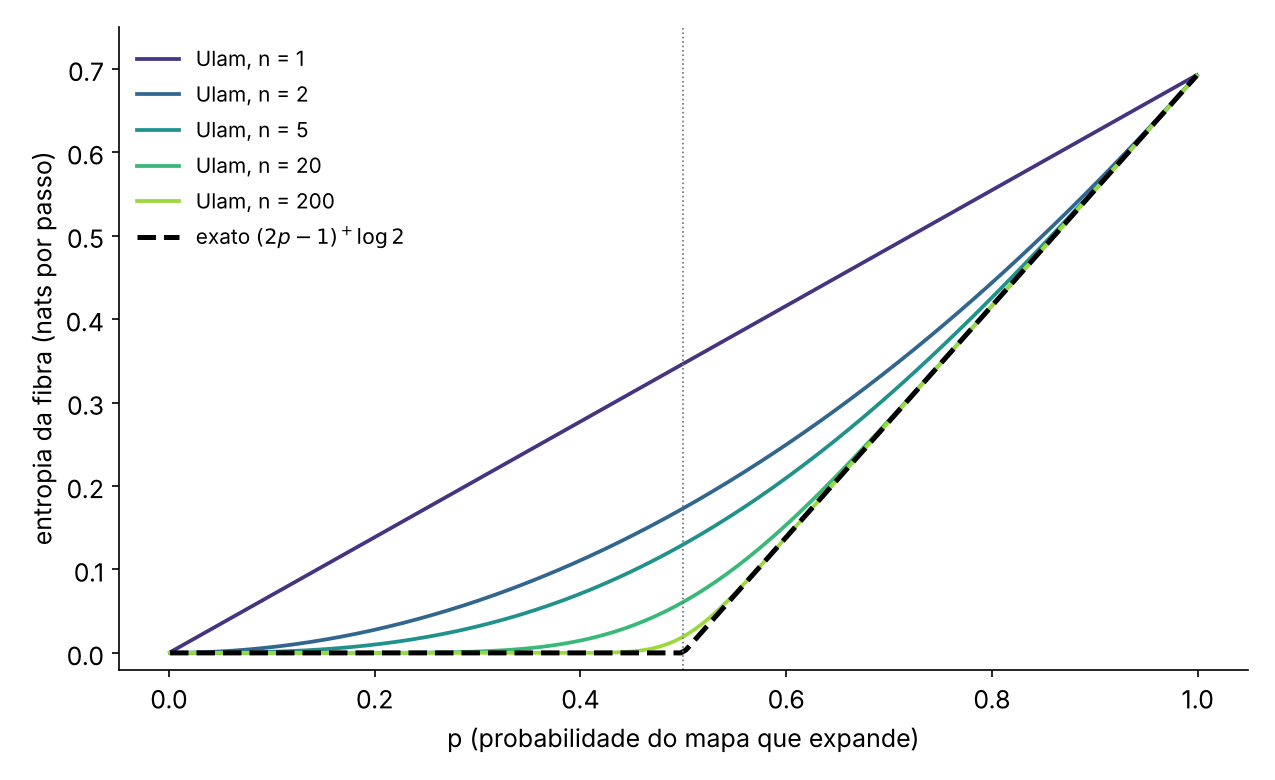
\includegraphics[width=0.72\linewidth]{figs/f7_principal.png}
  \caption{Estimador de Ulam $\hat h_n(p)$ para $n=1,2,5,20,200$ e valor exato
  $(2p-1)^+\log2$ (tracejado).}
  \label{fig:pelikan-principal}
\end{figure}

A Figura~\ref{fig:pelikan-conv} mostra a convergência em $n$ para valores fixos de $p$: longe
de $p=\tfrac12$ poucos passos bastam; em $p=\tfrac12$ a aproximação é a mais lenta.

\begin{figure}[ht]
  \centering
  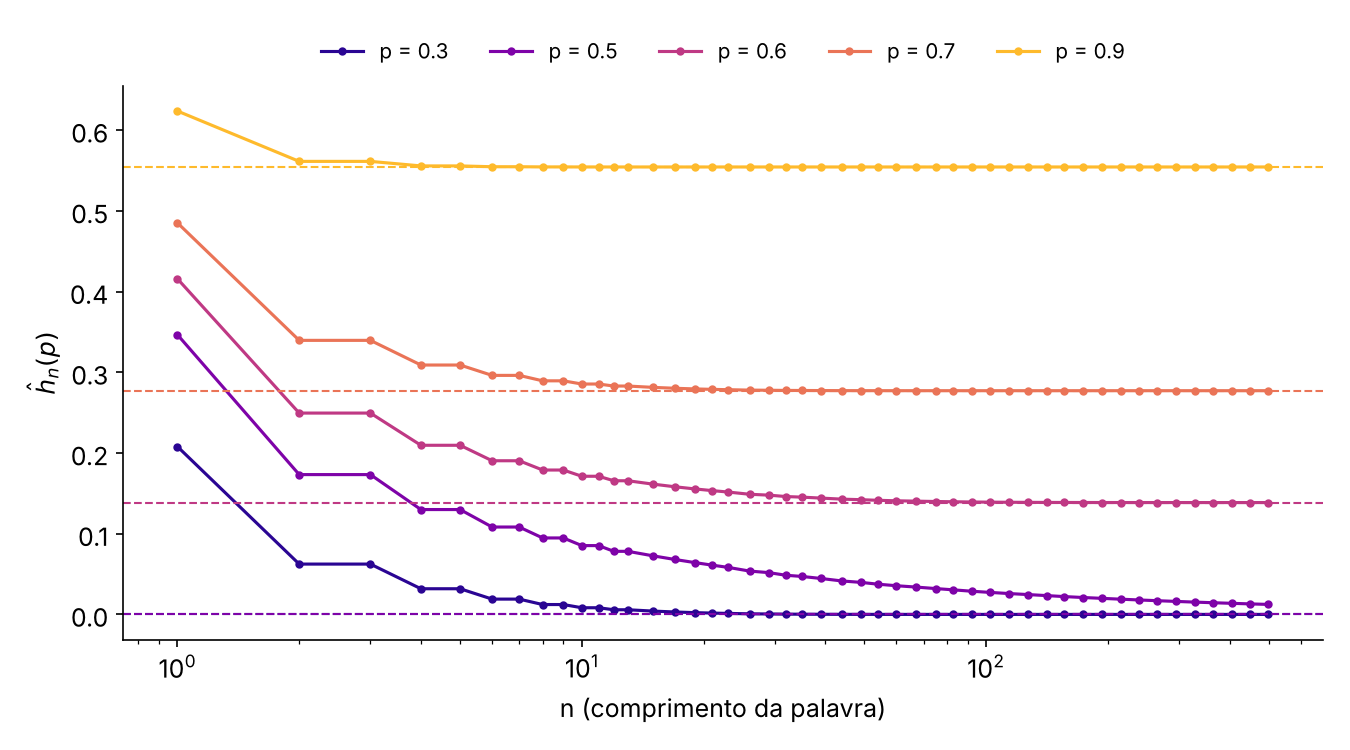
\includegraphics[width=0.75\linewidth]{figs/f9_convergencia_p.png}
  \caption{$\hat h_n(p)$ em função de $n$ para $p=0{,}3;\,0{,}5;\,0{,}6;\,0{,}7;\,0{,}9$. As linhas
  tracejadas são os valores exatos.}
  \label{fig:pelikan-conv}
\end{figure}

\paragraph{Como as curvas foram calculadas.} Para $n$ pequeno, as matrizes de Ulam foram
construídas diretamente (espalhando pontos em cada célula e aplicando os mapas). Para $n$
grande isso é inviável, pois há $2^n$ palavras; usamos então a fórmula fechada da
Seção~\ref{subsec:pelikan-geral}, que fornece \emph{exatamente} o mesmo valor que as matrizes.
A Tabela~\ref{tab:pelikan-conf} mostra a concordância para $n=4$.

\begin{table}[ht]
  \centering
  \begin{tabular}{ccc}
    \toprule
    $p$ & matrizes de Ulam ($n=4$) & fórmula fechada ($n=4$)\\
    \midrule
    0,3 & 0,03182 & 0,03182\\
    0,7 & 0,30907 & 0,30907\\
    0,9 & 0,55583 & 0,55583\\
    \bottomrule
  \end{tabular}
  \caption{Conferência entre as matrizes de Ulam construídas numericamente e a fórmula fechada.}
  \label{tab:pelikan-conf}
\end{table}

Por exemplo, para $p=0{,}7$: $\hat h_1=0{,}485$, $\hat h_2=0{,}340$, $\hat h_5=0{,}309$,
$\hat h_{20}=0{,}279$ e $\hat h_{200}=0{,}2773$, que já coincide com $0{,}4\log2\approx0{,}2773$.

% ---------------------------------------------------------------------
\subsection{Conclusões}

\begin{enumerate}
  \item \textbf{Precisão finita.} Em \texttt{double}, as órbitas deste sistema morrem em cerca de
        $53/(2p-1)$ passos; mais precisão só adia o problema. Métodos que dependem de órbitas
        longas não são confiáveis aqui.
  \item \textbf{Dois regimes.} Os mesmos dois mapas geram comportamentos opostos: para
        $p<\tfrac12$ as órbitas sincronizam, para $p>\tfrac12$ há dependência sensível. O que
        decide é o saldo entre expansões e contrações.
  \item \textbf{Método de Ulam.} O estimador mede o quanto as células se espalham usando poucos
        passos, e converge para $h_{\mathrm{fib}}(p)=(2p-1)^+\log2$, lentamente perto de
        $p=\tfrac12$. A média ingênua $p\log2$ está errada.
\end{enumerate}

% ---------------------------------------------------------------------
\subsection{Material complementar}

O repositório \url{\repoPelikan} contém:
\begin{itemize}
  \item o \emph{notebook} Jupyter que gera todas as figuras desta seção, com o código comentado e
        uma célula para experimentar outros valores de $p$ e $n$;
  \item os slides da apresentação (fonte \LaTeX{} e PDF).
\end{itemize}

\paragraph{Referências.}
\begin{itemize}
  \item Nota \emph{Ulam entropy} (material do curso), que contém a demonstração de que
        $h_{\mathrm{fib}}(p)=(2p-1)^+\log2$ e da fórmula fechada para $\hat h_n$.
  \item G.~Froyland, \emph{Ulam's method for random interval maps}, Nonlinearity \textbf{12}
        (1999), 1029--1052.
  \item C.~Monthus, \emph{Explicit dynamical properties of the Pelikan random map in the chaotic
        region and at the intermittent critical point towards the non-chaotic region},
        J.~Stat.~Mech.\ (2025), 013212.
  \item G.~Froyland, O.~Junge, G.~Ochs, \emph{Rigorous computation of topological entropy with
        respect to a finite partition}, Physica D \textbf{154} (2001), 68--84.
\end{itemize}
